\chapter{The Three-Body Problem}
\label{chap:three-body-problem}

Two bodies under mutual gravity trace conic sections: ellipses, parabolas,
hyperbolas, and rectilinear collision orbits as degenerate limiting cases.
Three bodies do not admit a comparable closed-form solution, a universal
one-dimensional radial reduction, or generic integrability. What survives is a
rich phase-space geometry: rotating-triangle exact solutions, equilibrium
points in the rotating frame, resonant islands, chaotic scattering, and
long-time transport.

Sundman (1907 announcement, 1912 publication) constructed a convergent series
solution away from triple collision.  The result is a remarkable existence
theorem, but it does not restore practical integrability or a usable
closed-form classification of motion. Binary collisions can be regularized by
changing variables and time scale. In the planar problem, the Levi-Civita change
\[
  z=u^2,\qquad \dd t=|u|^2\,\dd s
\]
turns the inverse-square collision singularity into a regular passage in the
\(u\)-plane: since \(|z|=|u|^2\), the singular potential \(1/|z|\) becomes
\(1/|u|^2\), and multiplication by the Sundman time factor
\(\dd t/\dd s=|u|^2\) cancels the leading pole. Equivalently, in the fixed-energy
Jacobi form, multiplying the Kepler expression \(T-GMm/|z|-E\) by \(|u|^2\)
turns the singular potential term into the smooth constant \(-GMm\). Sundman's
construction combines this local regularization with analytic continuation and
a global time reparametrization. Triple collision is the obstruction left out
of the global statement, and Belorizky emphasized in 1930 that Sundman's series
converges far too slowly for practical computation.

This chapter connects every phenomenon back to a controlled reduction of
Newton's law. We first formulate the full Newtonian three-body problem and
reduce translations using Jacobi coordinates. We then derive the circular
restricted three-body problem as a controlled limit and compute its
rotating-frame Hamiltonian, Jacobi constant, zero-velocity curves, and Lagrange
points. Finally we connect that model to the Sun-Jupiter-asteroid demo and to
ejection statistics.

\paragraph{Roadmap.}
The chapter moves through three models in a fixed order. The full three-body
problem supplies the Hamiltonian, the conserved quantities, and the reason
generic integrability fails. The circular restricted three-body problem supplies
the rotating frame, Jacobi constant, zero-velocity curves, and Lagrange points.
The heliocentric Sun-Jupiter-asteroid model supplies the finite-time ensemble
experiment. Each model keeps part of the previous one and discards part of it;
the text names those decisions so that numerical ejection is tied to a specified
model and time scale.

\paragraph{Model hierarchy.}
The reader should keep four levels separate:
\[
\begin{array}{rcl}
\text{two-body Kepler} &:& \text{integrable reference problem},\\
\text{full three-body} &:& \text{Newtonian Hamiltonian with all masses active},\\
\text{CR3BP} &:& \text{two primaries prescribed, one massless test body},\\
\text{asteroid ensemble} &:& \text{finite-time numerical statistic}.
\end{array}
\]
The later levels are controlled reductions chosen to isolate transport, escape
channels, and resonance-driven loss in a teachable setting.

\paragraph{Dimension convention.}
The phrase ``three-body problem'' by itself does not specify dimension.  The
Newtonian equations make sense for \(q_i\in\R^d\), with the physically spatial
case \(d=3\).  The planar problem, \(d=2\), is an invariant subproblem when the
initial positions and velocities lie in one plane; it is not a different force
law.  This chapter uses the spatial problem when discussing angular-momentum
geometry, hierarchical triples, and the general Newtonian formulation.  It uses
planar reductions for the CR3BP figures, the Sun-Jupiter-asteroid ensemble, the
equal-mass laboratory, and the current binary-scattering benchmark. Whenever a
numerical figure or probability estimate appears, the caption and surrounding
prose state whether the underlying run is planar or spatial.

\section{Astrophysical Regimes Of The Three-Body Problem}
\label{sec:three-body-astrophysical-regimes}

The three-body problem is not only a Solar-System problem.  It is the first
gravitational problem in which exact Keplerian integrability is generically
lost, and for that reason it appears throughout astrophysics.  The same
mechanical questions recur in different asymptotic regimes: Which two-body
orbit is the reference problem?  Which small parameter makes the motion nearly
integrable?  Which resonances are slow?  Which invariant or approximate
invariant controls escape, capture, or long-time stability?

\paragraph{Local notation.}
The symbols in the table are observables or control parameters for different
experiments.  \(a_{\rm p}\) is a planetary semimajor axis,
\(a_{\rm bin}\) a binary semimajor axis, \(T_{\rm inst}\) an instability time,
\(\sigma_{\rm cap}\) a capture cross section, and
\(\widehat P_{\rm ej}(T)\) a finite-sample ejection estimator at time \(T\).
None of these numbers is model-independent without the ensemble and stopping
rule that define it.

\begin{center}
\small
\setlength{\tabcolsep}{3pt}
\begin{tabular}{@{}p{0.20\textwidth} p{0.27\textwidth} p{0.27\textwidth} p{0.14\textwidth}@{}}
\hline
regime & controlled limit & typical question & observable\\
\hline
Sun-Jupiter-asteroid &
massless asteroid, nearly Keplerian heliocentric orbit &
mean-motion resonance, eccentricity growth, finite-time loss &
\(\widehat P_{\rm ej}(T)\)\\
S-type planet in a binary &
planet orbits one star, \(a_{\rm p}/a_{\rm bin}\ll1\) &
how far can the companion star perturb the planet before instability? &
stable fraction, \(T_{\rm inst}\)\\
circumbinary planet &
planet orbits outside a stellar binary, \(a_{\rm bin}/a_{\rm p}\ll1\) &
where is the inner chaotic boundary? &
critical semimajor axis\\
hierarchical triple &
inner binary plus distant third body &
secular exchange of inclination and eccentricity &
\(e_{\max}\), secular timescale\\
binary-single scattering &
incoming body meets a bound pair &
flyby, capture, exchange, ionization, or collision &
\(\sigma_{\rm cap}\), \(\sigma_{\rm exch}\)\\
\hline
\end{tabular}
\end{center}

The dimensional convention for the rows is as follows.  The
Sun-Jupiter-asteroid demo is planar.  The S-type and circumbinary planetary
problems are spatial in general, although planar slices are common first
models.  The hierarchical-triple calculation is spatial because mutual
inclination is dynamical.  The binary-single benchmark in these notes is
planar, while stellar-dynamical scattering in general is spatial.

This table is a map, not a replacement for derivation.  The Sun-Jupiter-
asteroid model is the detailed numerical example in these notes because its
semimajor-axis resonances connect cleanly to the perturbation theory of
Chapter~\ref{chap:perturbation-chaos}.  Binary stars and hierarchical triples
are equally central applications of the same Newtonian structure.  A planet
around one star in a binary is close to a Kepler problem with a distant
periodic perturber.  A circumbinary planet is close to a Kepler problem around
the binary center of mass, with a time-dependent multipole perturbation from
the inner pair.  A hierarchical triple is close to two Kepler problems coupled
by secular torques; because mutual inclination is one of its essential
dynamical variables, the Lidov--Kozai discussion below is spatial even after
secular reduction.  A binary-single encounter is less nearly integrable during
close approach, but its outcomes are still classified by the binding energies
of the outgoing pairs.  The benchmark later in this chapter uses a coplanar
binary-single ensemble for speed and visual clarity; a production
stellar-dynamical scattering calculation would sample the full
three-dimensional orientation and impact-parameter geometry.

\begin{figure}[htbp]
\centering
\begin{tikzpicture}[x=0.78cm,y=1cm, >=Latex, font=\scriptsize]
  \tikzset{
    star/.style={circle, draw=orange!80!black, fill=orange!25, inner sep=1.5pt},
    body/.style={circle, draw=blue!70!black, fill=blue!15, inner sep=1.1pt},
    panel/.style={draw=gray!55, rounded corners=2pt, minimum width=3.0cm,
      minimum height=2.35cm}
  }
  \foreach \x/\title in {
    0/{restricted\\Solar System},
    3.45/{S-type\\binary planet},
    6.90/{circumbinary\\planet},
    10.35/{hierarchical\\triple},
    13.80/{binary-single\\scattering}}
  {
    \node[panel] at (\x,0) {};
    \node[align=center] at (\x,1.33) {\title};
  }

  \node[star] at (-0.45,0.18) {};
  \node[body] at (0.38,0.18) {};
  \draw[gray!60] (-0.45,0.18) circle (0.72);
  \fill[blue!70!black] (0.26,0.33) circle (1pt);
  \node[align=center] at (0,-1.05) {resonant\\transport};

  \node[star] at (3.02,0.12) {};
  \node[star] at (4.15,0.12) {};
  \draw[gray!60] (3.58,0.12) circle (0.58);
  \draw[blue!60!black] (3.02,0.12) circle (0.35);
  \fill[blue!70!black] (3.34,0.26) circle (1pt);
  \node[align=center] at (3.45,-1.05) {planet\\stability};

  \node[star] at (6.70,0.15) {};
  \node[star] at (7.10,0.15) {};
  \draw[gray!60] (6.90,0.15) circle (0.78);
  \fill[blue!70!black] (7.58,0.52) circle (1pt);
  \node[align=center] at (6.90,-1.05) {chaotic\\inner edge};

  \node[star] at (10.12,0.10) {};
  \node[star] at (10.52,0.10) {};
  \draw[gray!60] (10.32,0.10) ellipse (0.42 and 0.20);
  \draw[blue!60!black] (10.32,0.10) ellipse (0.92 and 0.55);
  \fill[blue!70!black] (11.08,0.40) circle (1pt);
  \node[align=center] at (10.35,-1.05) {secular\\eccentricity};

  \node[star] at (13.48,0.12) {};
  \node[star] at (13.90,0.12) {};
  \draw[gray!60] (13.69,0.12) ellipse (0.42 and 0.22);
  \draw[blue!70!black, ->] (12.70,-0.55) -- (13.22,-0.05);
  \draw[blue!70!black, ->] (14.15,0.35) -- (14.73,0.72);
  \fill[blue!70!black] (12.70,-0.55) circle (1pt);
  \node[align=center] at (13.80,-1.05) {capture or\\exchange};
\end{tikzpicture}
\caption{Five astrophysical regimes of the three-body problem.  The diagrams
look different, but the mechanical questions are the same: choose a reference
Kepler problem when one exists, identify the slow perturbations, and define a
finite-time stability, escape, capture, or exchange observable.}
\label{fig:three-body-astrophysical-regimes}
\end{figure}

The word probability must be read with this model dependence in mind.  In
binary-single scattering, a ``capture probability'' is not a number attached to
the binary alone.  It is a probability for a stated ensemble of incoming
speeds, impact parameters, binary phases, orientations, masses, stopping
times, and outcome criteria.  If \(b\) is the impact parameter and
\(v_\infty\) is the incoming speed at large separation, scattering studies
often report a cross section,
\[
  \sigma_{\rm cap}(v_\infty)
  =
  \int 2\pi b\,\dd b\,
  P_{\rm cap}(b,v_\infty,\text{phase data},\text{criterion}),
\]
or its Monte Carlo estimate for a specified sampling rule.  This is the same
logical structure as the asteroid ejection statistic later in this chapter:
first define the experiment, then estimate the fraction or cross section.
The phrase ``at large separation'' is important.  If a numerical experiment
starts the incoming body at a finite distance, the launch speed must be chosen
so that energy conservation gives the desired \(v_\infty\) after the bodies are
separated.  The word capture also carries a finite-time convention in a
conservative three-body calculation: a body that is bound at the stopping time
may later escape unless a dissipative mechanism or an additional long-time
stability criterion is included.

Appendix~\ref{app:three-body-numerics} records the numerical protocol behind
the last two levels: coordinate choices, event definitions, resonance windows,
uncertainty estimates, and convergence checks. The chapter introduces these
choices where they first affect the mechanics; the appendix gathers them in one
place for reproducibility.

\section{Hierarchical Triples And The Lidov--Kozai Mechanism}
\label{sec:lidov-kozai-mechanism}

The hierarchical-triple row of the preceding table has its own canonical
calculation.  This is a spatial three-dimensional problem: if the motion were
strictly planar, the mutual inclination \(i\) would be fixed at \(0\) or
\(\pi\), and the Lidov--Kozai exchange between inclination and eccentricity
would disappear.  Consider an inner Kepler pair with semimajor axis \(a_1\),
eccentricity \(e\), argument of periapse \(\omega\), and inclination \(i\)
relative to a distant outer orbit.  Assume
\[
  a_1\ll a_2,
  \qquad
  e_2=0,
  \qquad
  \frac{L_1}{L_2}\ll1,
\]
where \(a_2,e_2\) are the outer orbital elements and \(L_1,L_2\) are the
Kepler angular-momentum scales.  The last assumption is the test-particle
limit: the outer orbit supplies a fixed angular-momentum axis.  The question is
what remains after averaging over both mean anomalies.  The answer is a
one-degree-of-freedom Hamiltonian in which eccentricity and inclination
exchange periodically.

\paragraph{Local notation.}
The subscript \(1\) labels the inner orbit and \(2\) labels the outer orbit.
The angle \(\omega\) here is the argument of periapse, not an angular velocity
or the symplectic form.  The inclination \(i\) is measured between the inner
and outer orbital angular-momentum directions.  The variables \(j\) and \(j_z\)
introduced below are dimensionless angular-momentum quantities.

Let
\[
  j=\sqrt{1-e^2},
  \qquad
  h=j\cos i.
\]
Here \(j\) is the inner angular momentum divided by the circular angular
momentum at the same \(a_1\), and \(h\) is its component along the fixed outer
angular-momentum axis.  In Delaunay variables, \(j\) is proportional to the
action \(G_{\rm D}\), while \(h\) is proportional to the node action \(H_{\rm
D}\).  After double averaging, the longitude of the ascending node is cyclic,
so \(h\) is conserved.  This conservation law is sometimes called the Kozai
constant:
\[
  \boxed{\sqrt{1-e^2}\cos i=\text{constant}.}
\]
The name is historical; mechanically it is Noether's theorem for rotations
about the outer orbit's angular-momentum axis.

\begin{derivation}[Quadrupole-averaged Hamiltonian]
Let the outer angular-momentum direction be the \(z\)-axis.  In the
test-particle quadrupole limit, the averaged perturbing potential is, up to a
positive constant factor,
\[
  \mathcal H_{\rm LK}
  =
  1-6e^2-3h^2
  +15e^2\left(1-\frac{h^2}{j^2}\right)\sin^2\omega,
  \qquad
  j^2=1-e^2 .
\]
The constant factor fixes the secular time unit but not the phase portrait.
All symbols in this expression have a direct orbital meaning:
\(\omega\) is the inner argument of periapse, \(e\) is inner eccentricity,
\(j\) is normalized inner angular momentum, and
\(1-h^2/j^2=\sin^2 i\) is the squared mutual-inclination sine.  The canonical
pair is \((\omega,j)\), with \(h\) fixed.

Here is where the numerical coefficients in this formula come from.  Write the
inner position as
\[
  r=xP+yQ,
\]
where \(P\) is the unit vector toward periapse and \(Q\) is the unit vector
obtained by rotating \(P\) by \(90^\circ\) in the orbital plane.  For an ellipse
with semimajor axis \(a_1\),
\[
  x=a_1(\cos E-e),
  \qquad
  y=a_1\sqrt{1-e^2}\sin E,
  \qquad
  \dd M=(1-e\cos E)\,\dd E,
\]
where \(E\) is eccentric anomaly and \(M\) is mean anomaly.  Averaging over
the inner mean anomaly gives
\[
  \left\langle\frac{x^2}{a_1^2}\right\rangle
  =
  \frac12+2e^2,
  \qquad
  \left\langle\frac{y^2}{a_1^2}\right\rangle
  =
  \frac12(1-e^2),
  \qquad
  \left\langle xy\right\rangle=0.
\]
Therefore
\[
  \left\langle\frac{r^2}{a_1^2}\right\rangle
  =
  1+\frac32e^2 .
\]
If the line of nodes is used as the reference direction, then
\[
  P\cdot\hat z=\sin i\,\sin\omega,
  \qquad
  Q\cdot\hat z=\sin i\,\cos\omega,
\]
and hence
\[
  \left\langle\frac{(r\cdot\hat z)^2}{a_1^2}\right\rangle
  =
  \sin^2 i
  \left[
  \frac12+e^2\left(\frac52\sin^2\omega-\frac12\right)
  \right].
\]
The quadrupole term is obtained by expanding the distant perturber's potential
to second order in \(a_1/a_2\), dropping the monopole and dipole pieces, and
averaging the circular outer orbit.  After multiplying by a positive constant
and choosing the irrelevant additive constant conveniently, the dimensionless
Hamiltonian can be taken as
\[
  \mathcal H_{\rm LK}
  =
  -2\left\langle\frac{r^2}{a_1^2}\right\rangle
  +6\left\langle\frac{(r\cdot\hat z)^2}{a_1^2}\right\rangle .
\]
Substituting the two averages gives
\[
  \mathcal H_{\rm LK}
  =
  1-6e^2-3(1-e^2)\cos^2 i
  +15e^2\sin^2 i\,\sin^2\omega .
\]
Finally \(h=j\cos i\) and \(j^2=1-e^2\), so
\[
  (1-e^2)\cos^2 i=h^2,
  \qquad
  \sin^2 i=1-\frac{h^2}{j^2},
\]
which is the boxed expression above.

The same result may be checked against the vector form
\[
  \Phi_{\rm quad}
  \propto
  1-6e^2-3(\mathbf j\cdot \hat z)^2
  +15(\mathbf e\cdot \hat z)^2,
\]
where \(\mathbf j\) is the dimensionless angular-momentum vector and
\(\mathbf e\) is the eccentricity vector.  Since
\(\mathbf j\cdot\hat z=h\) and
\((\mathbf e\cdot\hat z)^2=e^2\sin^2 i\,\sin^2\omega\), the scalar Hamiltonian
above follows.
\end{derivation}

The reduced equations are
\[
  \dot j=-\pd_\omega\mathcal H_{\rm LK},
  \qquad
  \dot\omega=\pd_j\mathcal H_{\rm LK},
\]
after choosing the dimensionless secular time associated with the omitted
positive factor.  Thus the quadrupole Lidov--Kozai problem is integrable: one
degree of freedom, one Hamiltonian, and one parameter \(h\).  The motion is
nontrivial because \(e\) and \(i\) are tied by \(h=j\cos i\).  If \(e\)
increases, then \(j\) decreases, and \(\cos i=h/j\) changes.  The inner orbit
can become highly eccentric without any close encounter; the slow secular
torque transfers angular momentum between inclination and eccentricity.

\begin{derivation}[Critical inclination and maximum eccentricity]
Take an initially circular inner orbit, \(e_0=0\), with inclination \(i_0\).
Then
\[
  j_0=1,\qquad h=\cos i_0,
\]
and the initial Hamiltonian is
\[
  \mathcal H_0=1-3\cos^2 i_0.
\]
At the maximum eccentricity reached by a Lidov--Kozai cycle, the orbit passes
through \(\omega=\pi/2\) or \(3\pi/2\).  Setting
\(\mathcal H_{\rm LK}(e_{\max},\omega=\pi/2)=\mathcal H_0\) gives
\[
  1-6e_{\max}^2-3h^2
  +15e_{\max}^2\left(1-\frac{h^2}{1-e_{\max}^2}\right)
  =
  1-3h^2 .
\]
The nonzero-eccentricity branch satisfies
\[
  9-\frac{15h^2}{1-e_{\max}^2}=0,
\]
so
\[
  \boxed{
  e_{\max}
  =
  \sqrt{1-\frac{5}{3}\cos^2 i_0}.
  }
\]
This expression is real only when
\[
  \cos^2 i_0<\frac35,
  \qquad
  \arccos\sqrt{\frac35}<i_0<\pi-\arccos\sqrt{\frac35}.
\]
Thus, in degrees, the quadrupole Lidov--Kozai window for an initially circular
orbit is approximately
\[
  39.23^\circ<i_0<140.77^\circ .
\]
Outside this window, the circular orbit is stable against the quadrupole secular
eccentricity growth.
\end{derivation}

\begin{figure}[htbp]
\centering
\begin{tikzpicture}[x=1cm,y=1cm,>=Latex,font=\small]
  \draw[->] (-0.2,0) -- (5.0,0) node[right] {\(\omega\)};
  \draw[->] (0,-0.15) -- (0,3.1) node[above] {\(e\)};
  \foreach \x/\lab in {0/{\(0\)},1.57/{\(\pi/2\)},3.14/{\(\pi\)},4.71/{\(3\pi/2\)}}
    \draw (\x,0.06)--(\x,-0.06) node[below] {\lab};
  \draw[blue!70!black,thick]
    plot[smooth cycle] coordinates {
      (0.60,0.35) (1.05,1.55) (1.57,2.55) (2.10,1.55)
      (2.55,0.35) (2.10,0.12) (1.57,0.05) (1.05,0.12)
    };
  \draw[blue!70!black,thick]
    plot[smooth cycle] coordinates {
      (3.20,0.35) (3.65,1.55) (4.18,2.55) (4.70,1.55)
      (5.15,0.35) (4.70,0.12) (4.18,0.05) (3.65,0.12)
    };
  \draw[gray!65,dashed] (1.57,0) -- (1.57,2.8);
  \draw[gray!65,dashed] (4.18,0) -- (4.18,2.8);
  \node[blue!70!black,align=center,fill=white,inner sep=2pt] at (2.55,2.55)
    {libration islands\\around \(\omega=\pi/2,3\pi/2\)};
  \node[align=center] at (2.55,-0.68)
    {fixed \(h=\sqrt{1-e^2}\cos i\): eccentricity growth is inclination loss};
\end{tikzpicture}
\caption{Schematic Lidov--Kozai phase portrait at fixed \(h\).  The precise
contours are level sets of the quadrupole-averaged Hamiltonian; the islands
show the counter-intuitive secular route from inclined nearly circular motion
to high eccentricity.}
\label{fig:lidov-kozai-phase-portrait}
\end{figure}

There is a small numerical subtlety in plotting this reduced system.  The
argument of periapse \(\omega\) is not defined at exactly \(e=0\), even though
the limiting instability of the circular orbit is physically meaningful.  The
demo therefore reports a tiny regularizing eccentricity seed when the requested
initial condition is circular, monitors the Hamiltonian drift, and terminates
with an explicit boundary diagnostic if the computed \(j=\sqrt{1-e^2}\) leaves
the regular chart.  This is a coordinate issue in the secular model, not an
additional physical force.  The numerical trajectory in the demo is integrated
with classical fourth-order Runge--Kutta.  RK4 is transparent enough for a
lecture laboratory, but it is not symplectic and does not preserve
\(\mathcal H_{\rm LK}\) exactly.  The plotted orbit should therefore be read
together with the printed Hamiltonian drift; for longer integrations one should
repeat the run at smaller \(\Delta \tau\) and check convergence of that drift.

\begin{figure}[htbp]
\centering
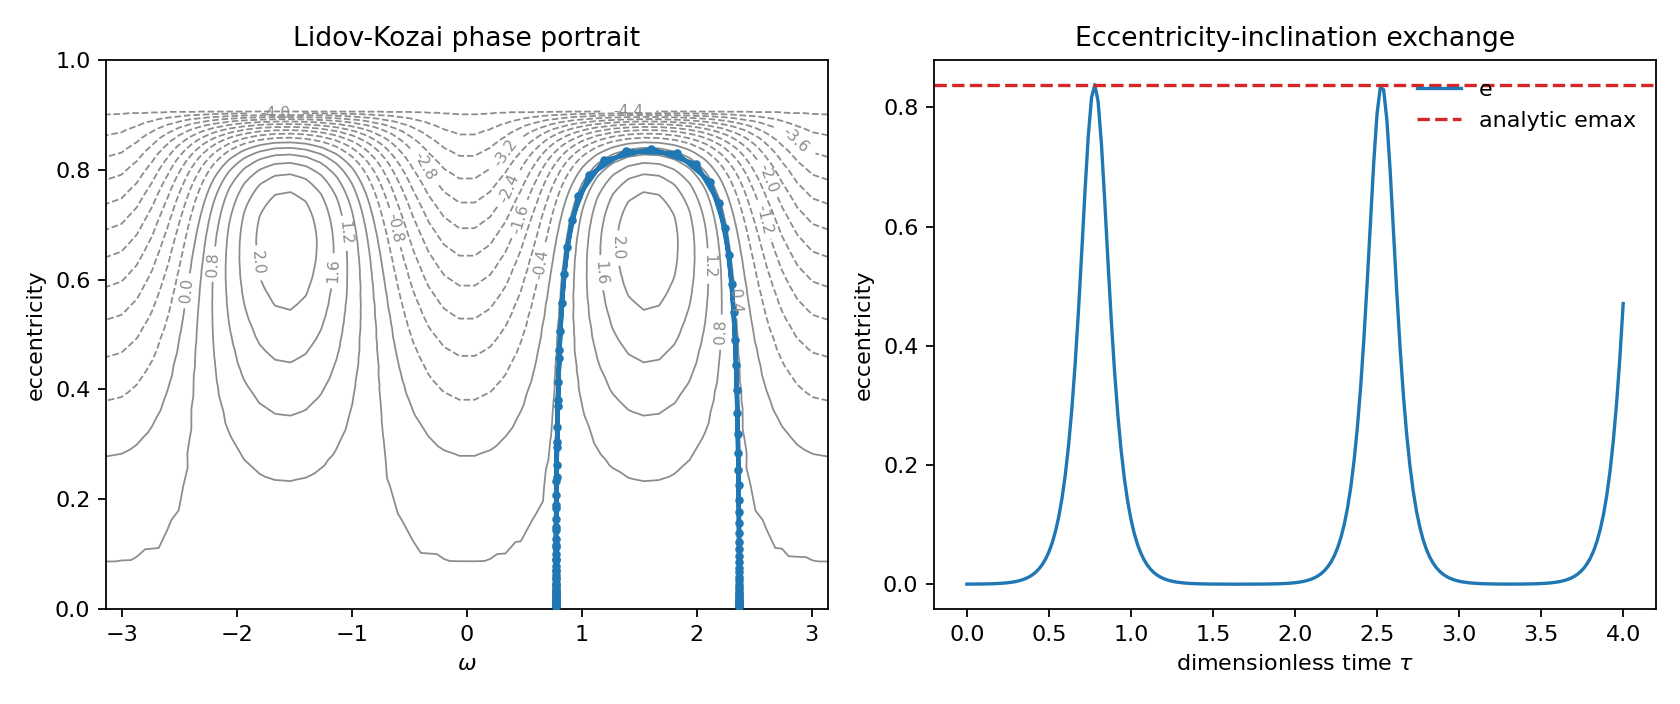
\includegraphics[width=0.96\textwidth]{../../figures/canonical/lidov_kozai_quick.png}
\caption{Numerical Lidov--Kozai laboratory generated by
\protect\path{demos/python/lidov_kozai.py} for an orbit initialized near
\(i_0=65^\circ\) with a tiny eccentricity seed.  The left panel is the reduced
phase portrait at fixed
\(h=\sqrt{1-e^2}\cos i\): the horizontal axis is the argument of periapse
\(\omega\) and the vertical axis is eccentricity \(e\).  Contours are level
sets of the quadrupole-averaged Hamiltonian, and the blue curve is one
numerically integrated secular trajectory on that same level-set geometry.  The
inline contour labels are numerical values of the dimensionless Hamiltonian
\(\mathcal H_{\rm LK}\) used by the script.  In the right panel the horizontal
axis is the script's dimensionless secular time \(\tau\), the vertical axis is
\(e(\tau)\), the blue curve is the numerical solution, and the dashed red line
is the analytic maximum
\(e_{\max}=\sqrt{1-(5/3)\cos^2 i_0}\).  The seed is a coordinate
regularization because \(\omega\) is undefined at exactly \(e=0\); it is not an
extra physical perturbation.}
\label{fig:lidov-kozai-numerical-lab}
\end{figure}

The lesson for the rest of the chapter is methodological.  A generic
three-body problem is not integrable, but a controlled hierarchical limit can
average to an integrable slow problem.  That slow problem can still produce a
large observable: high eccentricity, orbital flips in extended models, and
instability once short-range forces, octupole terms, tides, or encounters are
restored.

\paragraph{Historical context.}
Poincare's prize essay for King Oscar II's 1889 competition was substantially
revised after he discovered an error; Weierstrass, on the prize jury, demanded
a corrected version. The revision exposed homoclinic intersections and became
the foundation of \emph{Methodes nouvelles de la mecanique celeste}
(1892--1899). Birkhoff (1915) extended the program by making return maps and
periodic orbits operational tools of celestial mechanics. Painleve's 1895
singularity theorem clarified a separate issue: in the Newtonian three-body
problem, every finite-time singularity is caused by a collision. Xia's 1992
noncollision singularities for five bodies show that this is a special feature
of low \(N\), not a general safety theorem for Newtonian gravity.

\section{The Newtonian Three-Body Problem}
\label{sec:newtonian-three-body-problem}

The restricted problem will be derived as a limit of the Newtonian three-body
problem; we therefore start with the full problem.  Unless a planar reduction
is explicitly named, the equations in this section are the spatial equations
with \(q_i\in\R^3\).  The same force formula restricts consistently to
\(\R^2\) when all initial data are coplanar. The classical conserved
quantities, momentum, angular momentum, and energy, survive, but they no longer
reduce the dynamics to a one-dimensional radial equation. The restricted
problem is not a different force law; it is a controlled limit and coordinate
choice inside the same Newtonian interaction.

\paragraph{Local notation.}
The position \(q_i(t)\) and momentum \(p_i(t)\) belong to body \(i\), while
\(\mathbf r_{ij}=q_i-q_j\) is a relative vector and
\(r_{ij}=\norm{\mathbf r_{ij}}\) its length.  The total mass is
\(M=m_1+m_2+m_3\).  The total angular
momentum \(J\) should not be confused with the resonant action \(J\) used in
Chapter~\ref{chap:perturbation-chaos}.

Let \(q_i(t)\in\R^3\) be the inertial position of mass
\(m_i>0\), and write
\[
  \mathbf r_{ij}=q_i-q_j,\qquad r_{ij}=\norm{\mathbf r_{ij}}.
\]
The Lagrangian is
\[
  L(q,\dot q)
  =
  \sum_{i=1}^3 \frac12 m_i\norm{\dot q_i}^2
  +
  \sum_{1\leq i<j\leq 3}\frac{Gm_im_j}{r_{ij}},
\]
because \(L=T-V\) and the Newtonian potential energy is negative:
\[
  V(q)=-\sum_{i<j}\frac{Gm_im_j}{r_{ij}}.
\]
The Euler-Lagrange equation for \(q_i\) gives
\[
  m_i\ddot q_i
  =
  \sum_{j\neq i}
  Gm_im_j\frac{q_j-q_i}{\norm{q_j-q_i}^3}.
\]
After dividing by \(m_i\),
\[
  \boxed{
  \ddot q_i
  =
  \sum_{j\neq i}
  Gm_j\frac{q_j-q_i}{\norm{q_j-q_i}^3}.
  }
\]
This is a closed Hamiltonian system with canonical momenta \(p_i=m_i\dot q_i\)
and Hamiltonian
\[
  H(q,p)
  =
  \sum_{i=1}^3\frac{\norm{p_i}^2}{2m_i}
  -
  \sum_{i<j}\frac{Gm_im_j}{r_{ij}}.
\]

The center of mass
\[
  R_{\mathrm{cm}}=\frac{1}{M}\sum_i m_iq_i,
  \qquad
  M=m_1+m_2+m_3,
\]
moves uniformly because the internal gravitational forces cancel in pairs.
The total momentum, angular momentum, and energy are
\[
  P=\sum_i p_i,
  \qquad
  J=\sum_i q_i\times p_i,
  \qquad
  H=\text{constant}.
\]
These conserved quantities are essential, but they do not make the generic
three-body problem integrable. After removing center-of-mass motion, the
spatial problem has six relative configuration degrees of freedom and a
twelve-dimensional relative phase space. Fixing total angular momentum and
using rotational symmetry removes further dimensions, but not enough to leave a
one-degree radial problem. The planar invariant subproblem has four relative
configuration degrees of freedom and an eight-dimensional phase space. Fixing
the scalar angular momentum and quotienting the remaining planar rotation
removes two phase dimensions; a fixed-energy reduced space is still
five-dimensional.  Both the spatial and planar problems therefore have enough
room for separatrices, homoclinic tangles, chaotic scattering, and transport.

\subsection{Translation Reduction And Jacobi Coordinates}
\label{subsec:three-body-jacobi-coordinates}

The center-of-mass degree of freedom is dynamically trivial. Removing it shows
which variables remain in the interacting problem. The formulas below hold in
both \(d=3\) and \(d=2\): in the spatial problem the Jacobi vectors are in
\(\R^3\), while in the planar reduction they are in \(\R^2\). Let
\[
  m_{12}=m_1+m_2,\qquad M=m_{12}+m_3,
\]
and define Jacobi coordinates
\[
  R=\frac{m_1q_1+m_2q_2+m_3q_3}{M},
  \qquad
  \rho_1=q_2-q_1,
  \qquad
  \rho_2=q_3-\frac{m_1q_1+m_2q_2}{m_{12}}.
\]

\paragraph{Local notation.}
The coordinate \(R\) is the total center of mass, \(\rho_1\) is the separation
inside the pair \((1,2)\), and \(\rho_2\) points from that pair's center of
mass to body \(3\).  The reduced masses \(\mu_1\) and \(\mu_2\) belong to
these two Jacobi vectors; they are not the CR3BP mass parameter
\(\mu_{\mathrm{CR3BP}}\).

Here \(\rho_1\) is the relative vector inside the pair \((1,2)\), while
\(\rho_2\) points from the center of mass of that pair to the third body.  The
inverse transformation is
\[
\begin{aligned}
  q_1&=R-\frac{m_2}{m_{12}}\rho_1-\frac{m_3}{M}\rho_2,\\
  q_2&=R+\frac{m_1}{m_{12}}\rho_1-\frac{m_3}{M}\rho_2,\\
  q_3&=R+\frac{m_{12}}{M}\rho_2 .
\end{aligned}
\]
Substituting these expressions into the kinetic energy and collecting terms
gives the diagonal form
\[
  T=
  \frac12 M\norm{\dot R}^2
  +\frac12\mu_1\norm{\dot\rho_1}^2
  +\frac12\mu_2\norm{\dot\rho_2}^2,
  \qquad
  \mu_1=\frac{m_1m_2}{m_{12}},
  \qquad
  \mu_2=\frac{m_3m_{12}}{M}.
\]
The absence of cross terms is the point of Jacobi coordinates: the mass metric
has been diagonalized after translations are separated.

It is useful in celestial mechanics to write the attractive potential with a
positive sign,
\[
  U=-V>0.
\]
With this convention the Hamiltonian is kinetic minus attraction, \(H=T-U\).
The attraction potential becomes
\[
\begin{aligned}
  U(\rho_1,\rho_2)
  &=
  \frac{Gm_1m_2}{\norm{\rho_1}}
  +\frac{Gm_1m_3}
  {\norm{\rho_2+\frac{m_2}{m_{12}}\rho_1}}
  +\frac{Gm_2m_3}
  {\norm{\rho_2-\frac{m_1}{m_{12}}\rho_1}} .
\end{aligned}
\]
In the center-of-mass frame \(R=0\), the relative Hamiltonian is therefore
\[
  H_{\mathrm{rel}}
  =
  \frac{\norm{\pi_1}^2}{2\mu_1}
  +\frac{\norm{\pi_2}^2}{2\mu_2}
  -U(\rho_1,\rho_2),
\]
where \(\pi_a=\mu_a\dot\rho_a\).  This formula shows what
changed from the two-body problem: there are now two coupled relative vectors,
and each inverse-square attraction depends on a different linear combination of
them.

\begin{derivation}[Lagrange-Jacobi identity]
In the center-of-mass frame define the moment of inertia
\[
  I_{\mathrm{cm}}
  =
  \sum_{i=1}^3 m_i\norm{q_i}^2
  =
  \mu_1\norm{\rho_1}^2+\mu_2\norm{\rho_2}^2 .
\]
Differentiate once:
\[
  \dot I_{\mathrm{cm}}
  =
  2\sum_i m_i q_i\cdot\dot q_i,
\]
and then again:
\[
  \ddot I_{\mathrm{cm}}
  =
  4T+2\sum_i q_i\cdot m_i\ddot q_i .
\]
Since \(m_i\ddot q_i=\partial U/\partial q_i\) and \(U\) is homogeneous of
degree \(-1\), Euler's theorem gives
\[
  \sum_i q_i\cdot\frac{\partial U}{\partial q_i}=-U.
\]
Using \(H=T-U\) gives the two equivalent forms
\[
  \boxed{\ddot I_{\mathrm{cm}}=4T-2U=4H+2U.}
\]
This identity is a diagnostic for the size of the configuration. For a bounded
noncollisional motion, the long-time average of \(\ddot I_{\mathrm{cm}}\)
vanishes, so time averaging gives the virial relation
\(2\langle T\rangle=\langle U\rangle\).
For escape or near-collision, \(I_{\mathrm{cm}}\) instead records the large-scale
expansion or collapse of the configuration.
\end{derivation}

\begin{remark}[Why the two-body reduction does not generalize]
For two bodies, the center-of-mass reduction leaves one relative vector in a
central potential. Angular momentum reduces the dynamics to a one-dimensional
radial problem, while the Laplace-Runge-Lenz vector gives the conic orbit
because the inverse-square potential has a hidden Kepler symmetry. Central
forces alone do not give that vector; generic central potentials still precess.
For three bodies there is no single relative radius and no central force after
reduction. Pairwise forces keep changing the effective center seen by each
body, so the Kepler-only constants are no longer constants of the full motion.
\end{remark}

\subsection{Central Configurations And Special Solutions}
\label{subsec:central-configurations}

Some exact motions survive this complexity. A configuration
\(a_1,a_2,a_3\), with center of mass at the origin, is a central configuration
if there is a scalar \(\lambda\) such that
\[
  \sum_{j\neq i}
  Gm_j\frac{a_j-a_i}{\norm{a_j-a_i}^3}
  =
  -\lambda a_i
  \qquad
  (i=1,2,3).
\]

\paragraph{Local notation.}
The vectors \(a_i\) are a fixed shape, not the instantaneous positions
\(q_i(t)\).  The scalar \(\lambda\) sets the angular frequency of the rigidly
rotating solution after the overall scale is chosen.  Central configurations
are special shapes inside the full configuration space.
For three bodies, the noncollinear central configurations span a plane, and the
collinear ones lie on a line.  Thus the classical Lagrange and Euler examples
below are planar special motions even when they are embedded in the spatial
\(\R^3\) problem.

Then the ansatz
\[
  q_i(t)=R(\omega t)a_i
\]
solves the equations in a plane provided \(\omega^2=\lambda\). The shape
rotates rigidly even though the force law is gravitational.

\begin{example}[Lagrange equilateral solution]
Place three bodies at the vertices of an equilateral triangle and choose the
center of mass as origin. The gravitational force on each body points toward
the center of mass, so the central-configuration equation holds. For three
equal masses \(m\) and side length \(s\), the force on one mass has magnitude
\[
  2\frac{Gm^2}{s^2}\cos\frac{\pi}{6}
  =
  \sqrt3\,\frac{Gm^2}{s^2}.
\]
The distance from a vertex to the centroid is \(s/\sqrt3\). Equating this to
the centripetal force \(m\omega^2s/\sqrt3\) gives
\[
  \omega^2=\frac{3Gm}{s^3}.
\]
This is a genuine three-body orbit with fixed shape.
\end{example}

Lagrange found the equilateral family in 1772; the collinear configurations
were Euler's, from 1767. Both are finite-mass ancestors of the Lagrange points
in the restricted problem.

\begin{example}[Euler collinear solutions]
There are also central configurations with the three bodies on one line. The
relative separations are fixed in a rotating frame, and the line rotates
uniformly. Unlike the equilateral case, the ratios of the two gaps depend on
the three masses and are determined by an algebraic equation. These collinear
solutions are the ancestors of \(L_1,L_2,L_3\) in the restricted problem.
For the ordering \(m_1,m_2,m_3\) on a line, set the distance \(m_2m_3\) equal
to \(x\) times the distance \(m_1m_2\). Euler's calculation gives the quintic
\[
\begin{aligned}
 &(m_1+m_2)x^5+(3m_1+2m_2)x^4+(3m_1+m_2)x^3\\
 &\qquad -(m_2+3m_3)x^2-(2m_2+3m_3)x-(m_2+m_3)=0.
\end{aligned}
\]
Its unique positive root gives the gap ratio for that ordering; the other two
collinear configurations come from the other orderings of the masses.

Here is the reduction behind the polynomial. Place the bodies at
\[
  q_1=0,\qquad q_2=d,\qquad q_3=d(1+x),
\]
and subtract the center-of-mass acceleration, since a central configuration is
allowed to translate uniformly before the rotating-frame description is chosen.
The central-configuration equation says that the gravitational acceleration of
each body differs from the common center-of-mass acceleration by
\(-\omega^2(q_i-q_{\mathrm{cm}})\). Taking the difference of the equations for
\((q_2,q_1)\) and for \((q_3,q_2)\) eliminates the center-of-mass acceleration
and leaves two expressions for the same \(\omega^2\). Equating them, clearing
the denominators \(d^2\), \(x^2d^2\), and \((1+x)^2d^2\), and collecting powers
of \(x\) gives the displayed quintic. Explicitly, with the common factor
\(G/d^2\) suppressed,
\[
\begin{aligned}
  a_2-a_1
  &=
  -(m_1+m_2)
  +m_3\left(\frac1{x^2}-\frac1{(1+x)^2}\right),\\
  a_3-a_2
  &=
  m_1\left(1-\frac1{(1+x)^2}\right)
  -\frac{m_2+m_3}{x^2}.
\end{aligned}
\]
The central-configuration condition requires \(a_3-a_2=x(a_2-a_1)\). Multiplying
this equation by \(x^2(1+x)^2\) produces the quintic above. Thus \(x\) is the
only shape variable, while \(d\) sets the overall scale.
\end{example}

Section~\ref{sec:lab-three-body} turns the equal-mass equilateral solution into
a numerical laboratory. There the exact rotating triangle is used as the
comparison orbit, and small perturbations of the initial velocities show how a
central configuration can organize nearby motion without making the full
three-body problem integrable.
Chenciner and Montgomery (2000) discovered the figure-eight periodic orbit:
three equal masses chase one another along a single planar curve, with zero
total angular momentum. It is not a central configuration, and like Lagrange's
and Euler's solutions it does not make the generic three-body problem
integrable. Special exact orbits can exist without integrability.

\section{Circular Restricted Three-Body Problem}
\label{sec:circular-restricted-three-body-problem}

This section treats the planar CR3BP.  The primaries move on a circular orbit
in the \(x\)-\(y\) plane, and the test particle is also restricted to that
plane.  There is also a spatial CR3BP, with a third coordinate \(z\) and
vertical motion; it has the same rotating-frame origin and a Jacobi integral,
but its phase space is six-dimensional instead of four-dimensional.  The
figures and numerical demo in these notes use the planar version.

The local symbols in the circular restricted problem differ from the
heliocentric asteroid notation used later.  The two primaries have masses
\(m_1,m_2\), the dimensionless mass parameter is
\(\mu_{\mathrm{CR3BP}}=m_2/(m_1+m_2)\), and the test-particle coordinates in
the rotating barycentric frame are \(r=(x,y)\).  The distances from the test
particle to the primaries are \(r_1\) and \(r_2\), and
\(\Omega_{\mathrm{eff}}\) is the effective potential in the rotating frame.
This \(\Omega_{\mathrm{eff}}\) is not an angular velocity.

The circular restricted three-body problem is the standard autonomous model
behind the Sun-Jupiter-asteroid story. Two massive primaries move on circular
Kepler orbits about their common center of mass, and a third body has zero
mass, so it feels the primaries but does not affect them. This is the setting
of Jacobi's integral (1836) and of Hill's lunar restricted problem (1878), and
the setting in which Birkhoff's periodic-orbit program made return maps and
periodic points operational. After choosing units
in which
\[
  G(m_1+m_2)=1,\qquad
  \text{primary separation}=1,\qquad
  \text{angular speed}=1,
\]
define the mass parameter
\[
  \mu_{\mathrm{CR3BP}}=\frac{m_2}{m_1+m_2},
  \qquad
  0<\mu_{\mathrm{CR3BP}}\leq \frac12.
\]
In the uniformly rotating barycentric frame the primaries are fixed at
\[
  P_1=(-\mu_{\mathrm{CR3BP}},0),
  \qquad
  P_2=(1-\mu_{\mathrm{CR3BP}},0).
\]
For compactness in this section write \(\mu=\mu_{\mathrm{CR3BP}}\). If the
test particle has rotating-frame position \(r=(x,y)\), set
\[
  r_1=\sqrt{(x+\mu)^2+y^2},
  \qquad
  r_2=\sqrt{(x-1+\mu)^2+y^2}.
\]
The effective potential is
\[
  \boxed{
  \Omega_{\mathrm{eff}}(x,y)
  =
  \frac12(x^2+y^2)
  +
  \frac{1-\mu}{r_1}
  +
  \frac{\mu}{r_2}.
  }
\]
The first term is the centrifugal potential; the last two are the gravitational
potentials of the fixed primaries.

\begin{derivation}[Rotating-frame equations]
Let \(\rho(t)=R(t)r(t)\) be the inertial position, where \(R(t)\) rotates with
angular velocity \(\hat z\). Differentiating twice gives
\[
  \ddot\rho
  =
  R(t)\left(
    \ddot r+2\hat z\times\dot r+\hat z\times(\hat z\times r)
  \right).
\]
In the plane, \(\hat z\times(\hat z\times r)=-r\). The inertial gravitational
acceleration, expressed in the rotating frame, is
\[
  - (1-\mu)\frac{r-P_1}{r_1^3}
  - \mu\frac{r-P_2}{r_2^3}
  =
  \nabla\left(\frac{1-\mu}{r_1}+\frac{\mu}{r_2}\right).
\]
Therefore
\[
  \ddot r+2\hat z\times\dot r-r
  =
  \nabla\left(\frac{1-\mu}{r_1}+\frac{\mu}{r_2}\right),
\]
equivalently
\[
  \boxed{
  \ddot r+2\hat z\times\dot r=\nabla\Omega_{\mathrm{eff}}(r).
  }
\]
The last step moves the centrifugal term \(-r\) to the right-hand side and uses
\(\nabla[\frac12(x^2+y^2)]=r\).
In components,
\[
  \boxed{
  \ddot x-2\dot y=\Omega_x,
  \qquad
  \ddot y+2\dot x=\Omega_y.
  }
\]
The Coriolis force is velocity dependent and does no work in the rotating
frame, but the deeper reason a Jacobi integral exists is that the rotating-frame
Hamiltonian is autonomous. The conserved quantity is rotating-frame energy,
equivalently inertial energy minus \(\omega L_z\) in dimensional variables.
\end{derivation}

\begin{figure}[htbp]
\centering
\begin{tikzpicture}[scale=1.25, >=Latex]
  \draw[->] (-2.25,0) -- (2.45,0) node[right] {\(x\)};
  \draw[->] (0,-1.72) -- (0,1.74) node[above] {\(y\)};
  \coordinate (pone) at (-0.55,0);
  \coordinate (ptwo) at (1.05,0);
  \coordinate (lone) at (0.62,0);
  \coordinate (ltwo) at (1.52,0);
  \coordinate (lthree) at (-1.62,0);
  \coordinate (lfour) at (0.25,1.386);
  \coordinate (lfive) at (0.25,-1.386);
  \fill[yellow!80!black] (pone) circle (3.5pt);
  \node[yellow!45!black, below=5pt] at (pone) {\(P_1\)};
  \fill[orange!80!black] (ptwo) circle (2.6pt);
  \node[orange!80!black, below=5pt] at (ptwo) {\(P_2\)};
  \foreach \pt/\lab/\anchor in {lone/L_1/above left,ltwo/L_2/above right,lthree/L_3/above}
  {
    \draw[red!75!black, thick] (\pt) ++(0,-0.08) -- ++(0,0.16);
    \node[red!75!black, \anchor=3pt] at (\pt) {\(\lab\)};
  }
  \foreach \pt/\lab/\anchor in {lfour/L_4/above right,lfive/L_5/below right}
  {
    \draw[red!75!black, thick] (\pt) ++(-0.08,-0.08) -- ++(0.16,0.16);
    \draw[red!75!black, thick] (\pt) ++(-0.08,0.08) -- ++(0.16,-0.16);
    \node[red!75!black, \anchor=3pt] at (\pt) {\(\lab\)};
  }
  \draw[blue!60!black, ->] (1.28,-0.92) arc (-35:35:1.05);
  \node[blue!60!black, fill=white, inner sep=1pt] at (1.78,-1.18)
    {rotating frame};
\end{tikzpicture}
\caption{Circular restricted three-body geometry in rotating barycentric
coordinates. The primaries are fixed, while the test particle moves under
gravity, centrifugal force, and Coriolis deflection.}
\label{fig:cr3bp-rotating-frame}
\end{figure}

\begin{derivation}[Jacobi integral]
Dot the rotating-frame equation with \(\dot r\):
\[
  \dot r\cdot\ddot r
  +
  2\dot r\cdot(\hat z\times\dot r)
  =
  \dot r\cdot\nabla\Omega_{\mathrm{eff}}.
\]
The Coriolis term vanishes because \(\dot r\cdot(\hat z\times\dot r)=0\). Hence
\[
  \frac{\dd}{\dd t}\left(\frac12\norm{\dot r}^2\right)
  =
  \frac{\dd}{\dd t}\Omega_{\mathrm{eff}}(r(t)).
\]
Therefore
\[
  \frac12\norm{\dot r}^2-\Omega_{\mathrm{eff}}=\text{constant}.
\]
It is customary to multiply by \(-2\) and define the Jacobi constant
\[
  \boxed{
  C_J=2\Omega_{\mathrm{eff}}(x,y)-(\dot x^2+\dot y^2).
  }
\]
This is the energy integral of the autonomous rotating-frame problem.
Equivalently, before nondimensionalizing the angular speed to one, the
conserved rotating-frame Hamiltonian is the inertial energy shifted by
\(-\omega L_z\); the Jacobi constant is the customary sign-reversed version of
that autonomous Hamiltonian.
\end{derivation}

\begin{derivation}[Canonical Hamiltonian in the rotating frame]
The rotating-frame equations also come from a genuine autonomous Hamiltonian,
but the canonical momenta are not the velocity components.  The Lagrangian per
unit test-particle mass is
\[
  L_{\mathrm{rot}}
  =
  \frac12(\dot x^2+\dot y^2)
  +x\dot y-y\dot x
  +\Omega_{\mathrm{eff}}(x,y).
\]
The linear velocity term is the Coriolis term in variational form.  Hence
\[
  p_x=\frac{\partial L_{\mathrm{rot}}}{\partial\dot x}=\dot x-y,
  \qquad
  p_y=\frac{\partial L_{\mathrm{rot}}}{\partial\dot y}=\dot y+x.
\]
Solving for velocity gives \(\dot x=p_x+y\) and \(\dot y=p_y-x\).  The
Legendre transform gives
\[
\begin{aligned}
  H_{\mathrm{rot}}
  &=
  p_x\dot x+p_y\dot y-L_{\mathrm{rot}}\\
  &=
  \frac12(p_x^2+p_y^2)+yp_x-xp_y
  -\frac{1-\mu}{r_1}-\frac{\mu}{r_2}.
\end{aligned}
\]
Equivalently,
\[
  H_{\mathrm{rot}}
  =
  \frac12\big((p_x+y)^2+(p_y-x)^2\big)
  -\Omega_{\mathrm{eff}}(x,y).
\]
Along solutions
\[
  C_J=-2H_{\mathrm{rot}}.
\]
This equality is often the safest way to translate between the geometric
zero-velocity picture and the canonical phase-space picture: velocities are
natural for drawing allowed regions, while \((x,y,p_x,p_y)\) are natural for
Hamiltonian perturbation theory and Poincare maps.
\end{derivation}

The Jacobi constant gives an immediate geometric constraint. Since the squared
speed is nonnegative,
\[
  \dot x^2+\dot y^2
  =
  2\Omega_{\mathrm{eff}}(x,y)-C_J
  \geq0.
\]
Thus the allowed region in the rotating plane is
\[
  2\Omega_{\mathrm{eff}}(x,y)\geq C_J,
\]
and curves satisfying
\[
  2\Omega_{\mathrm{eff}}(x,y)=C_J
\]
are zero-velocity curves. They are not physical walls; they are projections of
the energy surface to configuration space. A test particle cannot cross a
forbidden region because that would require imaginary speed. When the
zero-velocity neck near \(L_1\) or \(L_2\) opens, transport between regions
becomes possible. This is the rotating-frame picture behind many capture,
escape, and ejection mechanisms.
The allowed components are often called Hill regions. Near a secondary primary,
the small allowed lobe gives the Hill-sphere approximation used in celestial
mechanics: it is the configuration-space shadow of the same Jacobi-energy
constraint, not a literal material boundary.

\begin{figure}[htbp]
\centering
\begin{tikzpicture}[scale=1.0, >=Latex]
  \begin{scope}
    \fill[gray!22] (-2.0,-1.15) rectangle (2.0,1.15);
    \draw[->] (-2.0,0) -- (2.25,0) node[right] {\(x\)};
    \draw[->] (0,-1.25) -- (0,1.25) node[above] {\(y\)};
    \draw[blue!70!black, thick] (-0.75,0) ellipse (0.62 and 0.45);
    \draw[blue!70!black, thick] (0.88,0) ellipse (0.34 and 0.27);
    \fill[white] (-0.75,0) ellipse (0.60 and 0.43);
    \fill[white] (0.88,0) ellipse (0.32 and 0.25);
    \fill[yellow!80!black] (-0.75,0) circle (2.8pt);
    \node[yellow!45!black, below=4pt, fill=white, inner sep=1pt,
      font=\small] at (-0.75,0) {\(P_1\)};
    \fill[orange!80!black] (0.88,0) circle (2.2pt);
    \node[orange!80!black, below=4pt, fill=white, inner sep=1pt,
      font=\small] at (0.88,0) {\(P_2\)};
    \draw[red!75!black, thick] (0.2,-0.09) -- (0.2,0.09);
    \node[red!75!black, above=3pt, fill=white, inner sep=1.5pt,
      font=\small] at (0.2,0.09) {\(L_1\)};
    \node[align=center] at (0,-1.65) {neck closed\\separate allowed lobes};
  \end{scope}
  \begin{scope}[xshift=5.6cm]
    \fill[gray!22] (-2.0,-1.15) rectangle (2.0,1.15);
    \draw[->] (-2.0,0) -- (2.25,0) node[right] {\(x\)};
    \draw[->] (0,-1.25) -- (0,1.25) node[above] {\(y\)};
    \draw[blue!70!black, thick]
      (-1.45,0) .. controls (-1.25,0.78) and (-0.36,0.82) .. (0.28,0.28)
      .. controls (0.88,0.66) and (1.38,0.52) .. (1.55,0)
      .. controls (1.38,-0.52) and (0.88,-0.66) .. (0.28,-0.28)
      .. controls (-0.36,-0.82) and (-1.25,-0.78) .. (-1.45,0);
    \fill[white]
      (-1.28,0) .. controls (-1.12,0.62) and (-0.34,0.66) .. (0.28,0.17)
      .. controls (0.78,0.50) and (1.18,0.40) .. (1.34,0)
      .. controls (1.18,-0.40) and (0.78,-0.50) .. (0.28,-0.17)
      .. controls (-0.34,-0.66) and (-1.12,-0.62) .. (-1.28,0);
    \fill[yellow!80!black] (-0.75,0) circle (2.8pt);
    \node[yellow!45!black, below=4pt, fill=white, inner sep=1pt,
      font=\small] at (-0.75,0) {\(P_1\)};
    \fill[orange!80!black] (0.88,0) circle (2.2pt);
    \node[orange!80!black, below=4pt, fill=white, inner sep=1pt,
      font=\small] at (0.88,0) {\(P_2\)};
    \draw[red!75!black, thick] (0.2,-0.09) -- (0.2,0.09);
    \node[red!75!black, above left=4pt, fill=white, inner sep=1.5pt,
      font=\small] at (0.2,0.09) {\(L_1\)};
    \draw[red!75!black, thick] (1.18,-0.09) -- (1.18,0.09);
    \node[red!75!black, above right=4pt, fill=white, inner sep=1.5pt,
      font=\small] at (1.18,0.09) {\(L_2\)};
    \draw[red!75!black, ->] (0.2,-0.52) -- (0.2,-0.14);
    \node[align=center] at (0,-1.65) {neck open\\transport channel};
  \end{scope}
\end{tikzpicture}
\caption{Schematic zero-velocity curves in the rotating CR3BP plane. Gray
regions are forbidden by \(2\Omega_{\mathrm{eff}}<C_J\); white regions are
allowed projections of the energy surface. Changing \(C_J\) can open a neck
near \(L_1\), creating a channel between previously separated regions.}
\label{fig:cr3bp-zero-velocity-neck}
\end{figure}

\subsection{Lagrange Points}
\label{subsec:lagrange-points}

Equilibria in the rotating frame satisfy
\[
  \dot x=\dot y=\ddot x=\ddot y=0,
  \qquad
  \nabla\Omega_{\mathrm{eff}}(x,y)=0.
\]

\paragraph{Local notation.}
The points \(L_1,\ldots,L_5\) are fixed points in the rotating barycentric
coordinates of the CR3BP.  The symbol \(\mu\) in this subsection is the
dimensionless CR3BP mass parameter, and \(P_1,P_2\) are the fixed primary
locations defined in Section~\ref{sec:circular-restricted-three-body-problem}.

There are five such points. The collinear points \(L_1,L_2,L_3\) lie on the
\(x\)-axis and solve the scalar equation
\[
  x
  -
  (1-\mu)\frac{x+\mu}{|x+\mu|^3}
  -
  \mu\frac{x-1+\mu}{|x-1+\mu|^3}
  =
  0.
\]
The absolute values encode which side of each primary the point lies on. There
is one solution between the primaries, one to the right of \(P_2\), and one to
the left of \(P_1\).

The triangular points are explicit:
\[
  \boxed{
  L_4=\left(\frac12-\mu,\frac{\sqrt3}{2}\right),
  \qquad
  L_5=\left(\frac12-\mu,-\frac{\sqrt3}{2}\right).
  }
\]
At either point \(r_1=r_2=1\). Substituting \(L_4\), for example, gives
\[
\begin{aligned}
  \Omega_x
  &=
  x-(1-\mu)(x+\mu)-\mu(x-1+\mu)\\
  &=
  \left(\frac12-\mu\right)
  -(1-\mu)\frac12
  -\mu\left(-\frac12\right)
  =
  0,
\end{aligned}
\]
and similarly \(\Omega_y=0\). The gravitational and centrifugal forces balance
in the rotating frame.

\begin{remark}[Linear stability of \(L_4,L_5\)]
Linearizing about \(L_4\) or \(L_5\) gives stable oscillations when
\[
  \mu(1-\mu)<\frac{1}{27}.
\]
Here is the calculation. Write a perturbation as
\((\xi,\eta)\) around \(L_4\). At \(L_4\),
differentiate
\[
  \Omega_{\mathrm{eff}}
  =
  \frac12(x^2+y^2)
  +
  \frac{1-\mu}{r_1}
  +
  \frac{\mu}{r_2}
\]
twice. If \(X_1=x+\mu\), \(X_2=x-1+\mu\), and
\(m_1=1-\mu\), \(m_2=\mu\), then
\[
\begin{aligned}
  \Omega_{xx}
  &=
  1-\sum_{a=1}^2\frac{m_a}{r_a^3}
  +3\sum_{a=1}^2\frac{m_aX_a^2}{r_a^5},\\
  \Omega_{yy}
  &=
  1-\sum_{a=1}^2\frac{m_a}{r_a^3}
  +3\sum_{a=1}^2\frac{m_ay^2}{r_a^5},\\
  \Omega_{xy}
  &=
  3\sum_{a=1}^2\frac{m_aX_ay}{r_a^5}.
\end{aligned}
\]
At \(L_4\), \(r_1=r_2=1\), \(X_1=1/2\),
\(X_2=-1/2\), and \(y=\sqrt3/2\), so
\[
  \Omega_{xx}=\frac34,\qquad
  \Omega_{yy}=\frac94,\qquad
  \Omega_{xy}=\frac{3\sqrt3}{4}(1-2\mu).
\]
The linearized equations
\[
  \ddot\xi-2\dot\eta=\Omega_{xx}\xi+\Omega_{xy}\eta,\qquad
  \ddot\eta+2\dot\xi=\Omega_{xy}\xi+\Omega_{yy}\eta
\]
have characteristic polynomial
\[
  \lambda^4+\lambda^2+\frac{27}{4}\mu(1-\mu)=0.
\]
Put \(s=\lambda^2\). Then
\[
  s^2+s+\frac{27}{4}\mu(1-\mu)=0,
  \qquad
  s_\pm=
  \frac{-1\pm\sqrt{1-27\mu(1-\mu)}}{2}.
\]
All four eigenvalues are purely imaginary exactly when the two roots
\(s_\pm\) are real and negative. Since their sum is \(-1\) and their product
is positive for \(0<\mu<1\), this is equivalent to the discriminant condition
\[
  1-27\mu(1-\mu)\ge0.
\]
Equivalently, for \(\mu\leq 1/2\),
\[
  \mu<\mu_R
  =
  \frac12\left(1-\sqrt{\frac{23}{27}}\right)
  \approx 0.03852.
\]
The Sun-Jupiter value is about \(9.53\times10^{-4}\), far below this threshold.
Trojan motion near the triangular points is therefore stable in this
linearized nontrivial three-body setting.
The stability criterion was derived by Gascheau (1843) and Routh (1875); its
Solar System relevance was confirmed in 1906, when Max Wolf discovered the
first Trojan asteroid, 588 Achilles, near Jupiter's \(L_4\).
\end{remark}

\subsection{Connection To The Asteroid-Belt Model}
\label{subsec:cr3bp-to-asteroid-belt}

The CR3BP is autonomous in the rotating barycentric frame and has the Jacobi
constant. The ejection-probability demo uses a closely related heliocentric
form in which Jupiter is prescribed on a circular orbit and the asteroid is
integrated in Sun-centered coordinates. The two descriptions are related by a
time-dependent rotation and translation, but they emphasize different things:
\begin{itemize}
\item rotating barycentric CR3BP: Jacobi constant, zero-velocity curves, and
Lagrange points;
\item heliocentric asteroid ensemble: Kepler elements, resonance bins, and
finite-time ejection statistics.
\end{itemize}
Both are useful. The first gives the clean phase-space geometry of escape
channels. The second makes direct contact with semimajor axes, mean-motion
resonances, and the asteroid-belt simulations.

The CR3BP companion script computes \(L_1,\ldots,L_5\), plots representative
zero-velocity curves, and prints the drift of the Jacobi constant along the
numerical trajectory. Its time stepper is classical fourth-order Runge-Kutta:
this is transparent for a first classroom calculation, but it is not
symplectic and it does not preserve the Jacobi integral exactly. Long-time
transport claims should therefore be checked against the printed Jacobi drift
and, in research calculations, against a structure-aware integrator.

\section{Heliocentric Sun-Jupiter-Asteroid Equations}
\label{sec:restricted-sun-jupiter-asteroid}

In this section \(r\) is the asteroid position relative to the Sun, \(r_J(t)\)
is Jupiter's prescribed heliocentric position, \(a_J\) is Jupiter's orbital
radius, and \(n_J\) is Jupiter's mean motion.  The masses \(M_\odot\) and
\(M_J\) are the solar and Jovian masses.  The momentum \(p\) in
\(H_{\mathrm{hel}}(r,p,t)\) is the asteroid momentum per unit asteroid mass in
the chosen units; it should not be confused with the integer \(p\) used in a
\(p:q\) resonance label.
This section is planar: \(r,r_J,p\in\R^2\).  A spatial restricted asteroid
model would use \(r\in\R^3\), include inclination and nodal variables, and
change the resonance bookkeeping.  The repository ejection demo deliberately
uses the planar model so that mean-motion resonance, eccentricity growth, and
finite-time loss can be displayed with a small reproducible ensemble.

Let \(r\in\R^2\) be the asteroid position relative to the Sun. Jupiter is
prescribed by
\[
  r_J(t)=a_J(\cos n_Jt,\sin n_Jt),
  \qquad
  n_J^2=\frac{G(M_\odot+M_J)}{a_J^3}.
\]
In a heliocentric non-inertial frame, the asteroid acceleration is
\[
  \boxed{
  \ddot r
  =
  -\frac{GM_\odot r}{\norm r^3}
  -
  GM_J
  \left(
    \frac{r-r_J}{\norm{r-r_J}^3}
    +
    \frac{r_J}{\norm{r_J}^3}
  \right)
  }.
\]
The first term is solar gravity. The first part of the Jupiter term is direct
gravitational attraction to Jupiter. The final term is the indirect term caused
by the acceleration of the heliocentric frame.

Equivalently, the asteroid obeys the explicitly time-dependent Hamiltonian
\[
  H_{\mathrm{hel}}(r,p,t)
  =
  \frac12\norm p^2
  -
  \frac{GM_\odot}{\norm r}
  -
  \frac{GM_J}{\norm{r-r_J(t)}}
  +
  GM_J\frac{r\cdot r_J(t)}{\norm{r_J(t)}^3}.
\]
The last term is the potential whose gradient gives the indirect acceleration.
Because \(r_J(t)\) is periodic, this is a periodically forced one-particle
Hamiltonian. It can be made autonomous by adjoining the forcing phase
\(\phi=n_Jt\) and its conjugate action \(I_\phi\). With
\[
  r_J(\phi)=a_J(\cos\phi,\sin\phi),
\]
the extended Hamiltonian is
\[
  K(r,p,\phi,I_\phi)
  =
  H_{\mathrm{hel}}(r,p,\phi)+n_JI_\phi,
\]
so Hamilton's equation gives \(\dot\phi=\partial K/\partial I_\phi=n_J\). The
remaining equations are
\[
  \dot r=\pd_p H_{\mathrm{hel}},
  \qquad
  \dot p=-\pd_r H_{\mathrm{hel}},
  \qquad
  \dot I_\phi=-\pd_\phi H_{\mathrm{hel}}.
\]
Because \(I_\phi\) does not appear in \(H_{\mathrm{hel}}\), the equations for
\((r,p,\phi)\) reproduce exactly the original periodically forced
heliocentric system with \(\phi=n_Jt\).  The extra variable \(I_\phi\) is a
bookkeeping action: its evolution records the energy exchanged with the
periodic forcing phase.  The resulting autonomous system has more than one
degree of freedom and can exhibit resonance and chaotic transport.

\begin{derivation}[Indirect term]
Let \(x\) be the asteroid position in an inertial frame and \(x_\odot\) the Sun
position. The heliocentric vector is \(r=x-x_\odot\). Then
\[
  \ddot r=\ddot x-\ddot x_\odot.
\]
The direct Jupiter acceleration of the asteroid is
\[
  -GM_J\frac{x-x_J}{\norm{x-x_J}^3}.
\]
The acceleration of the Sun due to Jupiter is
\[
  \ddot x_\odot=
  GM_J\frac{x_J-x_\odot}{\norm{x_J-x_\odot}^3}
  =
  GM_J\frac{r_J}{\norm{r_J}^3}.
\]
Subtracting \(\ddot x_\odot\) produces the indirect term
\[
  -GM_J\frac{r_J}{\norm{r_J}^3}.
\]
\end{derivation}

\begin{remark}[Why the indirect term matters]
Omitting the indirect term corresponds to holding the Sun fixed while Jupiter
pulls on the asteroid. That is sometimes useful as a simplified classroom
model, but it is not the heliocentric form of the restricted three-body
problem. Including the indirect term ensures that the coordinate origin
accelerates exactly as the Sun does in the prescribed Sun-Jupiter motion.
\end{remark}

\section{From Resonance To Loss}
\label{sec:from-resonance-to-loss}

The phrase ``resonance causes ejection'' is too compressed.  In the
Sun-Jupiter-asteroid model, the typical chain of reasoning has several links:
\[
  \begin{gathered}
  \text{mean-motion commensurability}
  \longrightarrow
  \text{slow resonant angle}
  \longrightarrow
  \text{resonant island or chaotic layer}\\
  \longrightarrow
  \text{eccentricity growth}
  \longrightarrow
  \text{crossing or escape criterion}.
  \end{gathered}
\]
The nominal semimajor-axis location \(a_{p:q}\) identifies where a slow angle
can form; it is not itself a loss criterion.

\paragraph{Local notation.}
The initial semimajor axis \(a_0\) labels an ensemble member before integration,
whereas \(a(t)\) is the osculating semimajor axis inferred from the current
state.  The perihelion distance \(q_{\rm peri}\) should not be confused with a
configuration coordinate \(q^i\), and \(Q_{\rm aph}\) denotes aphelion distance.
The resonant integers \(p,q\) in \(\phi_{p:q}\) are not momenta.

For an osculating Kepler ellipse around the Sun, define perihelion and aphelion
distances by
\[
  q_{\rm peri}=a(1-e),
  \qquad
  Q_{\rm aph}=a(1+e).
\]
The orbit crosses the radial range of a planet with orbital radius \(a_P\) only
if
\[
  q_{\rm peri}\le a_P\le Q_{\rm aph},
\]
with additional phase and inclination conditions in a more realistic model.
For an asteroid interior to Jupiter, Jupiter crossing requires approximately
\[
  Q_{\rm aph}\gtrsim a_J.
\]
Mars or Earth crossing is instead controlled by the perihelion distance:
\[
  q_{\rm peri}\lesssim a_{\rm Mars}
  \quad\text{or}\quad
  q_{\rm peri}\lesssim a_\oplus .
\]
These inequalities are only crossing tests.  Actual collision, close
encounter, or ejection still depends on phase, encounter geometry, and the
chosen stopping rule.

The resonant angle from Chapter~\ref{chap:perturbation-chaos} gives the
dynamical diagnostic.  If
\[
  \phi_{p:q}=p\lambda_J-q\lambda-(p-q)\varpi
\]
librates over an interval of time, the asteroid is phase locked to the
resonance.  If \(\phi_{p:q}\) circulates but the eccentricity diffuses near
overlapping resonances or separatrices, the particle may still be transported.
Thus a good numerical report records more than the final alive/lost count: it
records the initial distance from nominal resonance, an eccentricity history or
maximum eccentricity, crossing thresholds, and the finite-time loss class.

\section{Numerical Ejection Probability}
\label{sec:numerical-ejection-probability}

The symbols in this section describe an ensemble rather than one trajectory.
\(N\) is the number of sampled asteroids, \(a_0\) is an initial semimajor axis,
\(T\) is the finite integration horizon, \(\tau_{\rm ej}\) is the first
ejection time, and \(\widehat P_{\rm ej}(T)\) is a Monte Carlo estimator for
the stated model and stopping rule.  The hat reminds the reader that the
quantity is estimated from a finite sample.

This section turns the qualitative phrase ``asteroids are lost near
resonances'' into a finite numerical experiment.  The experiment is not the real
asteroid belt.  It is a planar restricted Sun-Jupiter-asteroid model in which
Jupiter is prescribed, the asteroids are massless and noninteracting, and a
finite integration horizon is chosen before the run begins.  The numerical
object is therefore a finite-time probability for a specified ensemble and loss
rule.

The highlighted simulation samples \(N\) test particles.  Their initial
semimajor axes lie in
\[
  a_0\in[a_{\min},a_{\max}],
\]
with small eccentricities, random orbital phases, and random periapse
directions.  Each sampled Kepler ellipse is converted to a Cartesian
heliocentric state, evolved in Jupiter's time-dependent restricted field, and
assigned the first absorbing event it reaches: ejection, solar collision, close
encounter with Jupiter, or survival to the end of the run. Let \(T\) be the
integration horizon.

The workflow is:
\[
\begin{gathered}
\text{choose model and units}
\longrightarrow
\text{sample initial Kepler elements}
\longrightarrow
\text{convert to Cartesian states}\\
\longrightarrow
\text{integrate the restricted equations}
\longrightarrow
\text{apply a loss rule}
\longrightarrow
\text{estimate a finite-time fraction}.
\end{gathered}
\]
Every arrow is part of the definition of the reported probability.

\begin{definition}[Finite-time ejection probability]
For a specified model, sampling distribution, time step, and ejection criterion,
the finite-time ejection probability estimate is
\[
  \widehat P_{\mathrm{ej}}(T)
  =
  \frac{1}{N}
  \sum_{i=1}^{N}\mathbf 1\{\text{particle \(i\) is ejected before time \(T\)}\}.
\]
\end{definition}

The corresponding survival estimate is
\[
  \widehat S(T)=1-\widehat P_{\rm loss}(T),
\]
where ``loss'' may mean ejection alone or the union of ejection, close
encounter, and collision, depending on the stated experiment.  If a bin
\(B\) in initial semimajor axis contains \(n_B\) particles and \(e_B(T)\) of
them are ejected by time \(T\), the conditional finite-time estimate is
\[
  \widehat P_{\rm ej}(T\mid a_0\in B)=\frac{e_B(T)}{n_B}.
\]
The notation displays the dependence that ordinary prose often hides:
changing \(T\), the bin \(B\), the integrator, or the loss definition changes
the quantity being estimated.

\begin{remark}[Ejection criterion in the demo]
The Python demo counts a particle as ejected if it reaches a large heliocentric
radius or if its heliocentric two-body energy is positive after it has moved
outside Jupiter's orbital scale. In the default configuration this means
\[
  r>20\,\mathrm{AU}
  \quad\text{or}\quad
  E_{\odot}>0\ \text{and}\ r>a_J,
\]
with \(a_J=5.2044\,\mathrm{AU}\). The same run separately records close
approaches to Jupiter, using the default threshold \(0.03\,\mathrm{AU}\), and
collisions with the inner solar cutoff, using the default threshold
\(0.02\,\mathrm{AU}\).
\end{remark}

\(\widehat P_{\mathrm{ej}}(T)\) is not a property of the three-body problem in
isolation; it is a property of an experiment. Five inputs determine it:
\[
  \text{model}+\text{initial ensemble}+\text{time horizon}
  +\text{numerical method}+\text{loss criterion}.
\]
The same physical question with different choices yields different numerical
values.

The demo also labels each semimajor-axis bin by its nearest low-order interior
mean-motion resonance with Jupiter. The nominal resonance locations are
\[
  a_{p:q}=a_J\left(\frac{q}{p}\right)^{2/3},
  \qquad
  (p:q)\in\{3:1,5:2,7:3,2:1\}.
\]
These labels are a diagnostic overlay. A semimajor-axis bin is wider and cruder
than a resonance island, and the actual resonance width depends on eccentricity
and perturbation strength. The overlay asks whether large loss fractions cluster
near the same places where perturbation theory predicts slow resonant angles.
The upgraded diagnostic output also groups particles by nearest nominal
resonance and reports finite-time survival checkpoints.  Those checkpoints do
not extrapolate to infinite time; they show how the chosen ensemble empties
over the stated interval.

For a bin containing \(n_b\) sampled particles and \(e_b\) ejections, the
reported fraction is
\[
  \widehat p_b=\frac{e_b}{n_b}.
\]
If the particles in that bin are treated as independent Bernoulli trials, a
rough sampling uncertainty is
\[
  \operatorname{SE}(\widehat p_b)
  \approx
  \sqrt{\frac{\widehat p_b(1-\widehat p_b)}{n_b}}.
\]
This is only a Monte Carlo error bar for the chosen numerical experiment. It
does not measure modeling error, timestep error, or the long-time instability
of the idealized Hamiltonian system.

The same caution applies to binary capture probabilities.  If a binary-single
scattering calculation reports
\[
  \widehat P_{\rm cap}
  =
  \frac{N_{\rm cap}}{N},
\]
that number is meaningful only with the incoming velocity distribution,
impact-parameter sampling rule, binary elements, integration horizon, and
capture criterion.  If the sampling is uniform in area for
\(0\le b\le b_{\max}\), a corresponding cross-section estimate is
\[
  \widehat\sigma_{\rm cap}
  =
  \pi b_{\max}^2\,\frac{N_{\rm cap}}{N}.
\]
The asteroid ejection fraction and the binary capture cross section are
different physical observables, but they share the same statistical grammar:
specified ensemble first, number second.

It is useful to name the estimand before naming the estimator.  For an
asteroid ensemble \(\mathcal E\), loss rule \(\mathcal L\), and integration
horizon \(T\), the finite-time probability is
\[
  p_{\mathcal E,\mathcal L}(T)
  =
  \mathbb P_{\mathcal E}\{\tau_{\mathcal L}\le T\},
\]
where \(\tau_{\mathcal L}\) is the first time at which the loss rule is
satisfied.  A Monte Carlo run estimates this number for the stated model, not
for all asteroids and not for all future time.  A binary-scattering cross
section is analogous:
\[
  \sigma_A(v_\infty)
  =
  \int 2\pi b\,\dd b\;
  P_A(b,v_\infty,\text{phase data}),
\]
where \(A\) is a stated finite-horizon outcome such as capture, exchange, or
collision.  The symbol \(A\) is part of the definition: changing the stopping
time or the binding-energy criterion changes the cross section being
estimated.

Three uncertainties must therefore be kept separate.  Sampling uncertainty is
the randomness of the finite ensemble.  Discretization uncertainty is the
change produced by \(\Delta t\), integration method, and close-encounter
handling.  Model uncertainty is the gap between the simplified problem and the
astrophysical system it represents.  A standard error reports only the first
of these.  A convergence table and invariant-drift diagnostics address the
second.  The third is a modelling judgment and must be discussed in words.

\section{Benchmark Statistical Studies}
\label{sec:three-body-benchmark-statistics}

The repository now contains a compact benchmark driver whose purpose is
different from a smoke test.  A smoke test asks whether code runs and preserves
basic invariants.  A benchmark statistical study asks whether a stated ensemble
produces a reproducible finite-time observable with uncertainty estimates.

\paragraph{Local notation.}
In this section \(N\) is the number of trials in a stated ensemble,
\(N_{\rm loss}\) is the number of asteroid trials classified as lost,
\(N_{\rm cap}\) and \(N_{\rm exch}\) are scattering trials classified as
capture and exchange, and \(b_{\max}\) is the maximum impact parameter sampled
in the binary experiment.  The plotted error bars are sampling estimates, not
model uncertainties.

Figures~\ref{fig:three-body-asteroid-loss-benchmark}
and~\ref{fig:three-body-binary-scattering-benchmark} are intentionally
separate.  They are not two views of one simulation.  They are two independent
classroom experiments with the same statistical grammar: specify an ensemble,
integrate a three-body model, classify finite-time events, and estimate an
observable with sampling uncertainty.  The first figure is a planar restricted
asteroid-loss experiment.  The second is a planar Newtonian binary-single
scattering experiment.  The common lesson is methodological, not that the
physical systems are directly coupled.

\paragraph{Accelerated asteroid loss benchmark.}
The asteroid benchmark uses the same planar restricted model as the ejection
demo, but increases Jupiter's mass by a stated factor so that a short
classroom integration produces visible losses.  The output is not a
Solar-System probability; it is a controlled stress test of the resonance-loss
pipeline.

For the canonical quick-run figure, the script uses \(48\) asteroids per seed,
two seeds, \(T=12\) yr, \(\Delta t=0.04\) yr, eight semimajor-axis bins, and a
Jupiter mass multiplied by \(25\).  These choices are deliberately artificial:
the mass scaling increases scattering and resonance-driven loss enough that the
mechanism can be seen in a small lecture-note run.  For seeds \(s\in S\), the
code estimates
\[
  \widehat P_{\rm loss}(T)
  =
  \frac{\sum_{s\in S}N_{\rm loss}(s,T)}
       {\sum_{s\in S}N(s)}
\]
and the same quantity in semimajor-axis bins.  The binomial standard error
\[
  \widehat{\operatorname{se}}
  =
  \sqrt{\frac{\widehat p(1-\widehat p)}{N}}
\]
measures only sampling variation for the stated finite ensemble.  The benchmark
also reports resonance-labelled rows, so one can see whether the visible loss
is concentrated near the nominal resonant regions or instead spread through
the entire annulus.

\begin{figure}[htbp]
\centering
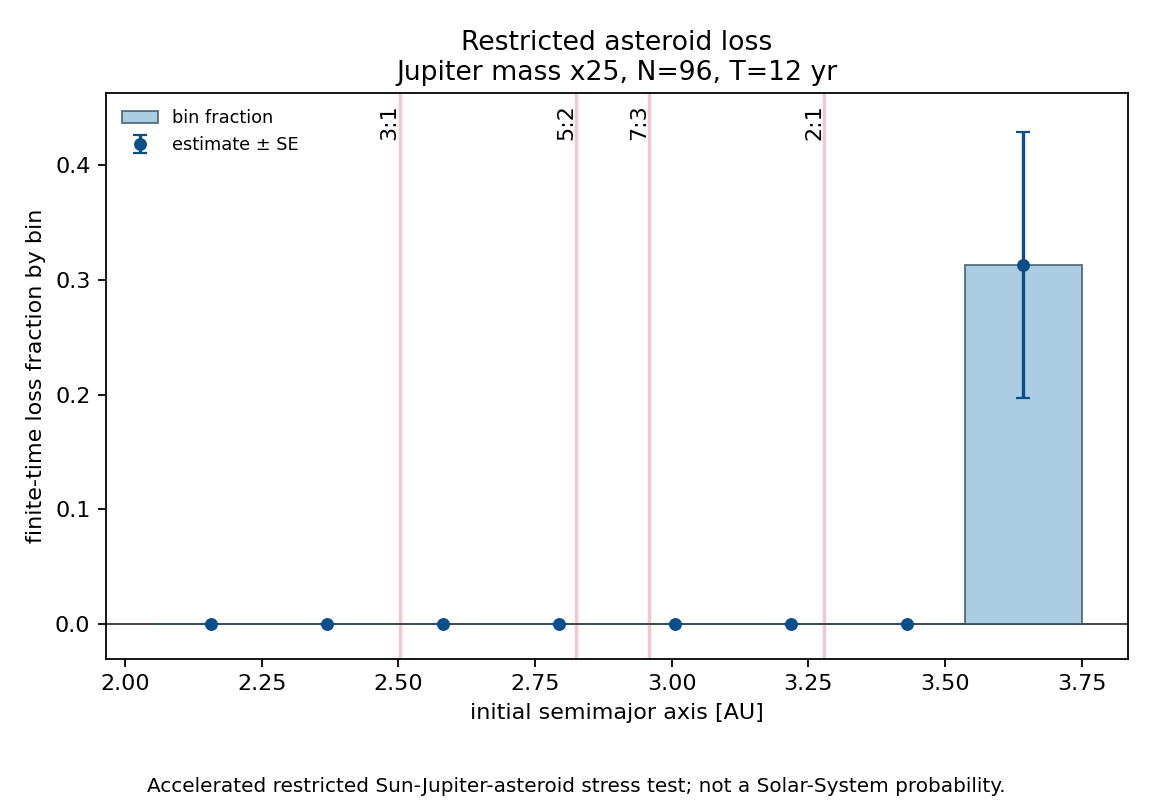
\includegraphics[width=0.78\textwidth]{../../figures/canonical/three_body_asteroid_loss_quick.png}
\caption{Accelerated restricted asteroid-loss benchmark generated by
\protect\path{demos/python/three_body_benchmark_studies.py}.  The horizontal axis is
the initial asteroid semimajor axis \(a_0\) in astronomical units, binned into
the displayed intervals.  The vertical axis is the finite-time loss fraction
in each bin after the stated integration horizon.  A loss means ejection,
collision with the Sun, or close approach to Jupiter according to the absorbing
rules in the script.  Each blue rectangle is one semimajor-axis bin: its width
is the bin interval in \(a_0\), and its height is the measured fraction
\(N_{\rm loss}/N_{\rm bin}\).  The blue dots mark the same bin estimates with
plug-in binomial standard-error bars; dots on the baseline are bins with
\(N_{\rm loss}=0\), for which the rectangle has zero height and the error
whisker has zero length.  Thus a dot sitting on the horizontal axis is not an
extra data set; it is the bin-center marker for a zero-loss bin.  In the quick
run shown here, the only nonzero bin is the last interval,
\(3.5375\,{\rm AU}\le a_0\le3.75\,{\rm AU}\), where \(5\) of \(16\) sampled
particles are lost, giving \(N_{\rm loss}/N_{\rm bin}=5/16=0.3125\).  The red
vertical lines mark nominal low-order Jovian resonances.  Jupiter's mass is
deliberately scaled up to make a short classroom run visibly lossy; the figure
is a stress test of the resonance-loss pipeline, not an estimate of the real
asteroid-belt loss probability.}
\label{fig:three-body-asteroid-loss-benchmark}
\end{figure}

\paragraph{Binary-single scattering benchmark.}
The binary benchmark sweeps over a small grid of incoming speeds
\(v_\infty\).  The canonical quick run uses an equal-mass circular binary
\((m_1,m_2)=(1,1)\) with \(a_{\rm bin}=1\), an incoming mass \(m_3=0.2\), launch
radius \(8a_{\rm bin}\), \(b_{\max}=1.5\), \(16\) samples per speed,
\(\Delta t=0.015\), and \(T=4\) in the binary units of the script.  The
benchmark is a planar Newtonian three-body calculation: all positions and
velocities have two components, and the binary and incoming body are coplanar.
It should not be read as a full spatial binary-single scattering survey.  In
the script's positive orientation the unshifted circular binary
has angular momentum in the \(+\hat z\) direction: if its separation vector is
\(a_{\rm bin}(\cos\phi,\sin\phi)\), its relative velocity is tangent to
increasing \(\phi\).  For each speed the code samples binary phase and impact
parameter.  With uniform-in-area sampling, it draws a random sign and
\(|b|=b_{\max}\sqrt{u}\) with \(u\) uniform on \([0,1]\).  Before subtracting
the total center of mass, the binary center of mass is placed at the origin and
the incoming body is launched from
\[
  q_3(0)=(-8a_{\rm bin},\,b),
  \qquad
  \dot q_3(0)=(v_{\rm launch},\,0),
\]
so the incoming trajectory is initially parallel to the positive \(x\)-axis and
the signed impact parameter \(b\) is the initial \(y\)-offset.  The binary
separation vector from body \(1\) to body \(2\) is
\[
  q_2(0)-q_1(0)
  =
  a_{\rm bin}(\cos\phi,\sin\phi),
\]
with \(\phi\) sampled uniformly in \([0,2\pi)\).  Thus Fig.~\ref{fig:three-body-binary-scattering-benchmark}
does not use one fixed binary orientation; it averages over binary orbital
phase at each \(v_\infty\).  By rotational invariance in the plane, sampling
\(\phi\) at fixed incoming direction is equivalent to fixing the binary phase
and sampling the incoming direction.  After this initialization the code
subtracts the total three-body center-of-mass position and velocity, which
changes neither relative orientation nor impact parameter.  The code chooses a
finite launch speed corresponding to the stated asymptotic \(v_\infty\),
integrates the planar Newtonian three-body equations, classifies finite-horizon
outcomes by pair binding energies, and reports
\[
  \widehat\sigma_{\rm cap/exch}(v_\infty)
  =
  \pi b_{\max}^2
  \frac{N_{\rm cap}+N_{\rm exch}}{N}
\]
for uniform-in-area sampling.  This \(\pi b_{\max}^2\) factor is an
axisymmetric area normalization attached to a planar trajectory ensemble; a
genuine three-dimensional scattering study would sample a two-component impact
parameter vector and the orientation of the binary plane relative to the
incoming direction.  The expected qualitative trend is that lower incoming
speeds have larger capture-or-exchange cross sections, because gravitational
focusing and longer interaction times make temporary binding easier.  The
benchmark is still a classroom calculation: capture means
``bound by the stopping-time classifier,'' not guaranteed permanent capture.

\begin{figure}[htbp]
\centering
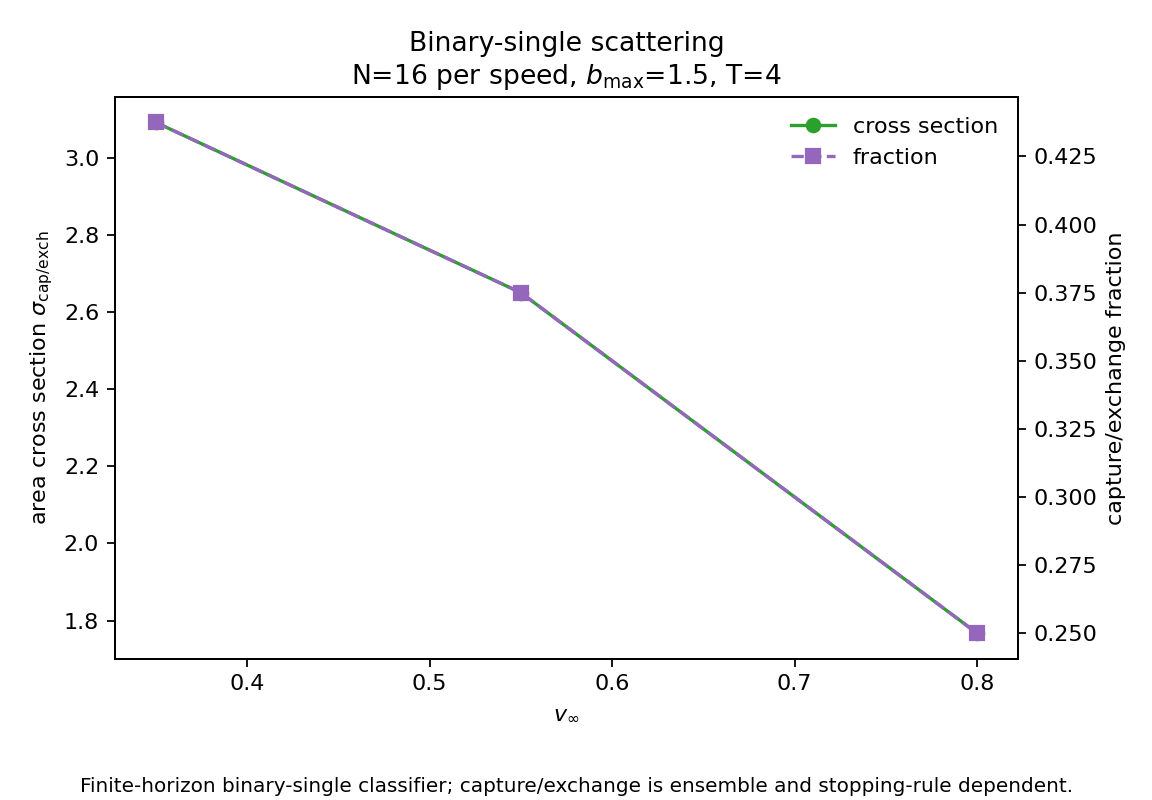
\includegraphics[width=0.78\textwidth]{../../figures/canonical/three_body_binary_scattering_quick.png}
\caption{Binary-single scattering benchmark generated by
\protect\path{demos/python/three_body_benchmark_studies.py}.  The horizontal axis is
the incoming speed \(v_\infty\) in the script's binary units.  For each value
of \(v_\infty\), the incoming body starts at \((-8a_{\rm bin},b)\) relative to
the binary center of mass and initially moves in the \(+x\) direction; the
binary orientation is the sampled phase
\(q_2-q_1=a_{\rm bin}(\cos\phi,\sin\phi)\), with \(\phi\) uniform on
\([0,2\pi)\).  The code then integrates the planar Newtonian three-body
equations and classifies the finite-horizon outcome using pair binding
energies.  The green curve uses the left vertical axis and plots the effective
capture-or-exchange cross section
\(\widehat\sigma_{\rm cap/exch}=\pi b_{\max}^2
(N_{\rm cap}+N_{\rm exch})/N\).  The purple dashed curve uses the right
vertical axis and plots the corresponding event fraction
\((N_{\rm cap}+N_{\rm exch})/N\).  The two vertical axes therefore show the
same event counts in two normalizations: fraction of sampled trials and
area-weighted cross section.  The two curves coincide by construction up to the
constant factor \(\pi b_{\max}^2\); the dual axis is a normalization of the
same estimator, not an independent measurement.  Capture here is a
finite-horizon classifier, not a claim of permanent astrophysical capture.}
\label{fig:three-body-binary-scattering-benchmark}
\end{figure}

Together these two studies turn the phrase ``three-body probability'' into a
specified data product.  The product contains the ensemble, the integration
horizon, the timestep, the event definition, the estimator, and the diagnostic
drifts.  Without that metadata, the reported number is not reproducible.

The figures should be read as model-audit devices.  In the asteroid-loss
figure, a visible bar asks for five checks before interpretation: how many
particles were
in the bin, what counted as loss, whether the bar is close to a meaningful
resonance marker, whether the loss persists under seed changes, and whether it
persists under timestep refinement.  In the scattering figure, the downward
trend with \(v_\infty\) is physically sensible because faster interlopers spend
less time in the strong-interaction region, but the plotted value is still
conditional on \(b_{\max}\), the phase distribution, the finite launch radius,
the stopping time, and the binding-energy classifier.  Neither panel should be
read without its metadata.

\section{Integrator Used In The Demo}
\label{sec:asteroid-integrator}

The demo uses a kick-drift-kick style update. If \(a(r,t)\) is the acceleration,
then
\[
\begin{aligned}
  v_{n+1/2} &= v_n+\frac{\Delta t}{2}a(r_n,t_n),\\
  r_{n+1} &= r_n+\Delta t\,v_{n+1/2},\\
  v_{n+1} &= v_{n+1/2}+\frac{\Delta t}{2}a(r_{n+1},t_{n+1}).
\end{aligned}
\]

\paragraph{Local notation.}
In this integrator formula \(a(r,t)\) is acceleration, not semimajor axis.
The integer \(n\) labels a time step, \(\Delta t\) is the fixed step size,
\(r_n\) and \(v_n\) are the asteroid position and velocity at step \(n\), and
\(v_{n+1/2}\) is an intermediate half-step velocity.

As written in physical time with prescribed Jupiter forcing, this update is not
the symplectic map of the autonomous extended Hamiltonian \(K\). It is still
pedagogically preferable to an opaque black-box integrator because every force
evaluation is visible.

The acceleration used in this update is the heliocentric restricted
acceleration displayed in Appendix~\ref{app:three-body-numerics}: solar
attraction, Jupiter's direct attraction, and the indirect term associated with
using the Sun as the origin.  The same timestep is used for all particles in one
run.  After each diagnostic step the code tests the absorbing loss rules; once a
particle is marked lost, it no longer contributes to later survival counts.  The
resulting probability estimate is therefore a property of the whole numerical
protocol: differential equation, timestep, stopping rule, and absorbing-event
bookkeeping.

\section{What To Take Forward}
\label{sec:three-body-take-forward}

\begin{itemize}
\item The full spatial three-body problem is Newtonian and Hamiltonian, with
positions \(q_i\in\R^3\).  Its planar subproblem, \(q_i\in\R^2\), is obtained
by choosing coplanar initial positions and velocities.  In neither version do
translation and rotation symmetries reduce the dynamics to a one-degree-of-freedom
radial equation.  The failure is structural, not a lack of clever
coordinates: Bruns proved in 1887, under algebraic hypotheses, that there are
no additional algebraic first integrals beyond the classical ones. Painleve's
work addressed a distinct question, the nature of finite-time singularities;
for the three-body problem such singularities are collision singularities.
Poincare's 1890 theorem addressed yet another class, ruling out generic
additional analytic integrals in the perturbative setting. The obstruction in
Poincare's setting is the same small-divisor mechanism seen in
Chapter~\ref{chap:perturbation-chaos}: a formal integral must solve
homological equations whose resonant denominators cannot be made to vanish
generically. These are not identical theorems with different names. Bruns
limits algebraic first integrals of the full problem, Painleve clarifies the
singularity structure, and Poincare explains why analytic integrability fails
under generic perturbation of an integrable model.
\item Jacobi coordinates remove center-of-mass motion and diagonalize the mass
metric.  They reveal two coupled relative vectors, which is the simplest
coordinate-level reason the two-body Kepler solution does not generalize.
\item Central configurations are exact special motions, not generic solutions.
They are valuable because they organize nearby dynamics and survive as
Lagrange-point structures in the restricted problem.
\item The circular restricted three-body problem used in this chapter is the
planar CR3BP: the primaries and massless particle move in one rotating plane,
and the phase space has coordinates \(x,y,\dot x,\dot y\).  It supplies an
autonomous rotating-frame model with Lagrange points, zero-velocity curves, a
canonical Hamiltonian, and the Jacobi constant. These structures are the
standard geometric language for capture and escape channels. The spatial CR3BP
adds vertical motion and a larger phase space.
\item The astrophysical three-body problem includes more than the Solar System.
Planets in binary-star systems, circumbinary planets, hierarchical triples, and
binary-single scattering all use the same ideas: a reference two-body motion
when one exists, a perturbing third body, resonant or secular exchange, and a
finite-time stability, capture, exchange, or ejection observable. Some of these
applications are intrinsically spatial, especially hierarchical triples with
inclination dynamics.  Planar slices remain useful when they are announced as
controlled reductions.
\item The Lidov--Kozai mechanism is the controlled spatial hierarchical-triple
example: double averaging leaves one slow degree of freedom, conserves
\(\sqrt{1-e^2}\cos i\), and predicts high eccentricity above the critical
inclination.  The symbol \(i\) is the mutual inclination of the inner and outer
orbits; without this three-dimensional angle, the effect disappears.
\item The heliocentric Sun-Jupiter-asteroid model in this chapter is a planar,
periodically forced Kepler problem.  Its indirect term is part of the
coordinate transformation, not an optional correction. A spatial asteroid model
would also track inclination and nodal variables.
\item A nominal resonance location is not a loss criterion.  Loss requires an
additional dynamical route, such as eccentricity growth to a crossing condition,
followed by the stated close-encounter, collision, or escape rule.
\item Numerical ejection, capture, and exchange probabilities are finite-time,
model-dependent observables. They become meaningful only when the dimension
of the phase space, the ensemble, integration time, timestep, invariant or
drift diagnostics, event classifier, and estimator are stated.
\end{itemize}

\section{Chapter-End Laboratories And Exercises}
\label{sec:three-body-chapter-end-labs}

This laboratory is the finite-mass counterpart of the restricted
Sun-Jupiter-asteroid simulations: derive Newton's equations, choose controlled
initial data, and monitor invariants before interpreting instability.

\subsection{Equal-Mass Three-Body Laboratory}
\label{sec:lab-three-body}

For an equal-mass three-body laboratory, take three masses in the plane with
pair potential
\[
  V=-k\left(\frac1{r_{12}}+\frac1{r_{23}}+\frac1{r_{13}}\right),
\]
where
\[
  r_{ij}=\norm{r_i-r_j}.
\]

\paragraph{Local notation.}
The vectors \(r_i\) in this laboratory are planar positions of the three equal
masses; they are not the relative separation \(r=x_1-x_2\) used in the Kepler
problem.  The constant \(k>0\) sets the gravitational coupling, and
\(\epsilon\) later denotes a small velocity perturbation.  This is a planar
finite-mass laboratory, not the full spatial three-body problem; the same
pair force can of course be written for \(r_i\in\R^3\).

The Lagrangian is
\[
  L=\sum_{i=1}^3\frac12m\norm{\dot r_i}^2
  +
  k\left(\frac1{r_{12}}+\frac1{r_{23}}+\frac1{r_{13}}\right).
\]
The equations are
\[
  m\ddot r_i
  =
  -k\sum_{j\neq i}\frac{r_i-r_j}{\norm{r_i-r_j}^3}.
\]
The symmetric initial positions are
\[
  r_1(0)=(1,0),
  \qquad
  r_2(0)=\left(-\frac12,\frac{\sqrt3}{2}\right),
  \qquad
  r_3(0)=\left(-\frac12,-\frac{\sqrt3}{2}\right).
\]

\begin{figure}[htbp]
\centering
\begin{tikzpicture}[scale=1.15, >=Latex, font=\small]
  \draw[->] (-2.0,0) -- (2.2,0) node[right] {\(x\)};
  \draw[->] (0,-1.7) -- (0,1.9) node[above] {\(y\)};
  \coordinate (r1) at (1.25,0);
  \coordinate (r2) at (-0.625,1.083);
  \coordinate (r3) at (-0.625,-1.083);
  \draw[gray!70, thick] (r1) -- (r2) -- (r3) -- cycle;
  \fill[blue!70!black] (r1) circle (2pt)
    node[above, fill=white, inner sep=1pt] {\(r_1\)};
  \fill[blue!70!black] (r2) circle (2pt)
    node[above left, fill=white, inner sep=1pt] {\(r_2\)};
  \fill[blue!70!black] (r3) circle (2pt)
    node[below left, fill=white, inner sep=1pt] {\(r_3\)};
  \draw[->, red!75!black, thick] (r1) -- ++(0,0.65);
  \draw[->, red!75!black, thick] (r2) -- ++(-0.56,-0.32);
  \draw[->, red!75!black, thick] (r3) -- ++(0.56,-0.32);
  \draw[dashed] (0,0) circle (1.25);
  \node[red!75!black, align=center, fill=white, inner sep=1.5pt] at (1.72,1.36)
    {tangent velocities\\for rotating triangle};
  \node[align=center, fill=white, inner sep=1.5pt] at (0,-1.95)
    {the perturbation lab changes the initial velocities\\and monitors
     energy, angular momentum, and separation};
\end{tikzpicture}
\caption{Equal-mass three-body laboratory. The unperturbed comparison solution
starts from an equilateral triangle with tangential velocities; perturbing this
initial data is a controlled way to watch the loss of symmetric motion.}
\label{fig:lab-three-body-initial-data}
\end{figure}
\FloatBarrier

For the rotating equilateral solution, velocities are tangent to the
circumcircle. A representative perturbed initial condition uses a speed
parameter \(v=0.8\) and perturbation \(\epsilon=0.05\), with initial velocities
such as
\[
  \dot x_1(0)=\epsilon,\qquad
  \dot x_2(0)=-\frac{\sqrt3}{2}v-\epsilon,\qquad
  \dot x_3(0)=\frac{\sqrt3}{2}v.
\]
The workflow matters more than the particular number \(0.8\): derive Newton's
equations from a Lagrangian, integrate the exact pairwise forces, monitor
energy and angular momentum, and compare unperturbed symmetric motion with
perturbed motion. This is the finite-mass cousin of the Sun-Jupiter-asteroid
ejection simulation.

\subsection{Questions For The Reader}
\label{sec:three-body-questions}

\begin{enumerate}
\item Starting from the inertial three-body Lagrangian, derive the
center-of-mass equation and explain why internal gravitational forces cancel in
pairs.
\item Verify the Jacobi-coordinate kinetic energy formula by substituting the
inverse transformation for \(q_1,q_2,q_3\). Which mass factors would be wrong
if the center of mass of bodies \(1\) and \(2\) were not used in \(\rho_2\)?
\item Use the homogeneity of \(U\) to rederive the Lagrange-Jacobi identity.
What does it imply for a bounded noncollisional orbit?
\item For the Sun-Jupiter value of \(\mu_{\mathrm{CR3BP}}\), where are
\(L_1,L_2,L_3\) relative to Jupiter?
\item For a chosen Jacobi constant, which zero-velocity necks are open?
\item Show explicitly that \(C_J=-2H_{\mathrm{rot}}\) after converting
canonical momenta to rotating-frame velocities.
\item How does \(\widehat P_{\mathrm{ej}}(T)\) change with \(T\)?
\item Which semimajor-axis bins have the largest ejection fractions?
\item What changes when \(M_J\) is scaled upward?
\item Which losses are close encounters, and which are clean ejections?
\item How sensitive are the results to \(\Delta t\)?
\item Are apparent resonance structures stable under a different random seed?
\item For an initially circular hierarchical triple, use the quadrupole
Lidov--Kozai Hamiltonian to derive
\[
  e_{\max}=\sqrt{1-\frac53\cos^2 i_0}\, .
\]
\item In Figure~\ref{fig:lidov-kozai-numerical-lab}, compare the numerical
maximum eccentricity with the analytic \(e_{\max}\).  Which part of the
comparison would fail if the plotted trajectory had large Hamiltonian drift?
\item In a binary-single scattering experiment, what information must be
specified before the phrase ``capture probability'' has a definite meaning?
\item For each numerical experiment in this chapter, identify whether the
integrated Cartesian state is planar or spatial.  Which quantities would have
to be added to turn the planar asteroid or binary-scattering demos into full
spatial ensembles?
\item If impact parameters are sampled uniformly in area for
\(0\le b\le b_{\max}\), derive
\(\widehat\sigma_{\rm cap}=\pi b_{\max}^2N_{\rm cap}/N\).
\item Use Figures~\ref{fig:three-body-asteroid-loss-benchmark}
and~\ref{fig:three-body-binary-scattering-benchmark} to separate sampling
statements from modelling statements.  Which uncertainty displayed in the
asteroid-loss figure comes from finite \(N\), and which questions require new
simulations rather than larger error bars?
\end{enumerate}

\section{Associated Demos}
\label{sec:three-body-demos}

\begin{itemize}
\item \path{demos/python/circular_restricted_three_body.py}.\\
Planar CR3BP.
\item \path{demos/python/lidov_kozai.py}.\\
Spatial hierarchical triple reduced by double averaging to one secular degree
of freedom.
\item \path{demos/python/asteroid_ejection_probability.py}.\\
Planar restricted Sun-Jupiter-asteroid ensemble.
\item \path{demos/python/asteroid_resonance_normal_form.py}.\\
Planar resonant normal-form calculation.
\item \path{demos/python/binary_capture_scattering.py}.\\
Planar Newtonian binary-single scattering, with the reported cross section
using the stated area normalization.
\item \path{demos/python/three_body_benchmark_studies.py}.\\
Planar asteroid and planar binary-scattering benchmark statistics.
\item \path{demos/mathematica/CircularRestrictedThreeBody.wl}.\\
Planar CR3BP.
\item \path{demos/mathematica/AsteroidEjectionProbability.wl}.\\
Planar restricted asteroid ensemble.
\item \path{demos/mathematica/AsteroidResonanceNormalForm.wl}.\\
Planar resonance-normal-form calculation.
\end{itemize}
Use the CR3BP demo first: it checks the Jacobi constant and draws the
zero-velocity geometry. Use the ejection-probability demo second: it turns the
same dynamical ideas into an ensemble statistic, so the meaningful outputs are
not only trajectories but also loss criteria, timestep sensitivity, resonance
bins, and finite-time uncertainty. Use the resonance-normal-form demo to see
the pendulum approximation behind resonance width. Use the binary-capture demo
as a parallel statistical experiment: its capture and exchange fractions are
not universal constants, but ensemble-dependent observables for the stated
planar scattering protocol. Use the Lidov--Kozai demo for the integrable
spatial secular hierarchical-triple limit, and use the benchmark driver when
the goal is an aggregate statistical result rather than a single smoke-test
trajectory. Figures~\ref{fig:lidov-kozai-numerical-lab},
\ref{fig:three-body-asteroid-loss-benchmark}, and
\ref{fig:three-body-binary-scattering-benchmark} are the reference visual
outputs for those uses.  Appendix~\ref{app:three-body-numerics}, especially
Section~\ref{sec:three-body-benchmark-figure-protocol}, records the numerical
protocol behind the benchmark figures.
